\documentclass[12pt, a4paper]{scrartcl}

% CONFIG
\newcommand{\exptitle}{Optisches Pumpen}       % long name of experiment 
\newcommand{\exptitleshort}{Optisches Pumpen} % short name of experiment
\newcommand{\expdate}{7. bis 17. April 2015}           % date of experiment
\newcommand{\exptutor}{Betreuer}

% PACKAGES + MODIFICATIONS
\usepackage[ngerman]{babel} %standard language stuff
\usepackage[T1]{fontenc}
\usepackage[utf8]{inputenc}
\usepackage{textgreek}

\usepackage[fleqn]{amsmath}  % math
\usepackage{amssymb}

\usepackage{graphicx} %graphics
\usepackage{float} 
\graphicspath{{../img/}}

\usepackage[automark,headsepline]{scrlayer-scrpage} %headings
\pagestyle{scrheadings}
\ihead{\exptitleshort}
\ohead{\pagemark}
\cfoot{}

\usepackage{hyperref}
\hypersetup{
    unicode=true,          % non-Latin characters in Acrobat’s bookmarks
    pdftoolbar=true,       % show Acrobat’s toolbar?
    pdfmenubar=true,       % show Acrobat’s menu?
    pdffitwindow=false,    % window fit to page when opened
    pdfstartview={FitH},   % fits the width of the page to the window
    pdfnewwindow=true,     % links in new window
    colorlinks=true,       % false: boxed links; true: colored links
    linkcolor=blue,       % color of internal links (change box color with linkbordercolor)
    citecolor=green,       % color of links to bibliography
    filecolor=magenta,     % color of file links
    urlcolor=blue          % color of external links
}

\usepackage[labelfont=bf]{caption} % bold captions

\usepackage{chngcntr} % change behaviour of counters in different environments
\counterwithin{figure}{section}  % number figures per section
\numberwithin{equation}{section} % number equations per section
\numberwithin{table}{section}    % number tables per section

\usepackage{enumerate} % better way to config enumerates

\setcounter{tocdepth}{2} % table of contents depth

\setlength{\parindent}{0pt} % no indent on new paragraph

\usepackage{pdfpages} % include pdf files

\usepackage{pdflscape} % landscape mode

% NEW COMMANDS

% DOCUMENT SETTINGS

\title{\exptitle}
\subtitle{Fortgeschrittenen-Praktikum 1}
\author{Moritz Bitterling und Benjamin Rottler \\ Universität Freiburg}
\date{\expdate}

% DOCUMENT
\begin{document}

\hypersetup{pageanchor=false} %stop page numbering (hyperref) to prevent for double page numers
\newcommand{\HRule}{\rule{\linewidth}{0.5mm}}
\begin{titlepage}
\begin{center}
  \textsc{\Large Fortgeschrittenen-Praktikum II}\\[0.5cm]
  \HRule \\[0.4cm]
  { \huge \bfseries \exptitle}\\
  \HRule \\[0.5cm]
  \large \expdate\\[0.5cm]  
  \begin{minipage}{0.4\textwidth}
    \begin{flushleft} \large
      Moritz \\ \textsc{Bitterling}
    \end{flushleft}
  \end{minipage}
  \hfill
  \begin{minipage}{0.4\textwidth}
    \begin{flushright} \large
      Benjamin \\ \textsc{Rottler}
    \end{flushright}
  \end{minipage}
  \\[1cm]
  \large 
  Betreuer: \exptutor \\[3cm]
  
\includegraphics[height=8cm]{../../img/logo_uni.pdf}
  \vfill
  \normalsize
  \textsc{Institut für Mathematik und Physik} \\
  \textsc{Albert-Ludwigs-Universität} \\
  \textsc{Freiburg im Breisgau}
\end{center}
\end{titlepage}
\thispagestyle{empty}

\newpage
Alle Berechnungen in diesem Protokoll wurden unter Python 3.4 mit Hilfe folgender Programmbibliotheken
\begin{itemize}
  \item PyROOT (\url{http://root.cern.ch/drupal/content/pyroot})
  \item NumPy (\url{http://www.numpy.org/})
\end{itemize}
oder mit oder Mathematica 10.0 durchgeführt. % TODO delete when Mathematica not used
Die Graphiken wurden mit Inkscape (\url{http://www.inkscape.org}) gezeichnet.\\[\baselineskip]
Alle Python-Skripte, \LaTeX-Skripte und SVG-Graphiken können online unter \\
\url{https://github.com/Bigben37/FP2/tree/master/0407-Optisches Pumpen} abgerufen werden. %TODO GitHub URL
\thispagestyle{empty}

\newpage
\tableofcontents
\thispagestyle{empty}

\newpage
\hypersetup{pageanchor=true} %start page numbering again
\setcounter{page}{1} %set to page 1

\section{Versuchsziel}
Im Versuch wird die Hyperfeinstruktur von Rubidium durch die Messung von Laserlichttransmission durch
gasförmiges Rubidium untersucht.
In verschiedenen Konfigurationen des Aufbaus werden Magnetfeldstärken und Anregungsfrequenzen variiert,
um die beiden Rubidiumisotope optisch zu pumpen und so Informationen über
den Kernspin, Relaxationszeiten und äußere Magnetfelder zu erhalten. 
\section{Physikalische Grundlagen}

3-4 Seiten, nur was für Auswertung relevant

1 Termschema

Diodenlaser, Modensprünge. Nix mit pn..

Zeeman, Hyperfein

Etalon

Spinpräzessionsfrequent, zwei $\alpha$s

\subsection{Spinpräzession des Rubidiumensembles im äußeren Magnetfeld}
Der Mechanismus der Spinpräzession wird in einem Versuchsteil ausgenutzt,
um die Stärke eines Magnetfelds sehr genau zu bestimmen.
Spinpräzession tritt auf, wenn ein Ensemble von Atomen im Magnetfeld optisch gepumpt,
das Ensemble also polarisiert wird, und anschließend eine Komponente
des Magnetfelds abgeschaltet wird (im Experiment die Komponente in Strahlrichtung).
Die Spins der Atome führen dann eine Präzessionsbewegung um das verbleibende Magnetfeld aus,
im Experiment ist das die Vertikalkomponente.
Die Präzessionsfrequenz beträgt (\cite{staatsex})
\begin{equation}
  f=\frac{g_\text{F} \cdot \mu_\text{B}}{h} \cdot B=: \beta \cdot B
\end{equation}




\subsection{Orientierungsprozesse im Rubidiumensemble}
In diesem Abschnitt wird ein kurzer Überblick über die mathematische Beschreibung der Orientierungsprozesse
(Polarisation und Relaxation) im Rubidiumgas gegeben und es werden die Zusammenhänge aufgeführt, die für die
Auswertung der Messungen zur Relaxationszeit notwendig sind.
Die ausführliche Herleitung der Formeln wird in \cite{staatsex} gezeigt.

Betrachtet man ein Ensemble von Rubidiumatomen, das im Magnetfeld durch zirkular polarisiertes Licht gepumpt wird,
wird die zeitliche Änderung der Differenz der Besetzungszahlen~$\left(\frac{\difd n}{\difd t}\right)_{\text{Pump}}$
durch die folgende Differenzialgleichung beschrieben:
\begin{equation}
  \left(\frac{\difd n}{\difd t}\right)_{\text{Pump}}=\frac{N-n}{T_\text{P}}
\end{equation}
$N$ ist die Anzahl der Atome im Ensemble, $n$ die Differenz der Besetzungszahlen in dem Zweiniveausystem
und $T_\text{P}$ die charakteristische Zeit für den Pumpvorgang, die \emph{Pumpzeit}.

Der Relaxationsvorgang wird durch folgende Differenzialgleichung beschrieben:
\begin{equation}
  \left(\frac{\difd n}{\difd t}\right)_{\text{Relax}}=-\frac{n}{T_\text{R}}
\end{equation}
$T_\text{R}$ ist die \emph{Relaxationszeit}.

Die Summe von Polarisation und Relaxation beschreibt den Orientierungsprozess im Rubidiumgas mit
der Orientierungszeit $\tau$:
\begin{equation}
\label{eq:orientierungszeit}
  \left(\frac{\difd n}{\difd t}\right)_{\text{Orient}}
  =\left(\frac{\difd n}{\difd t}\right)_{\text{Pump}} + \left(\frac{\difd n}{\difd t}\right)_{\text{Relax}}
  =\frac{N}{T_\text{P}}-n \left( \frac{1}{T_\text{P}} + \frac{1}{T_\text{R}}\right)
  =:\frac{N}{T_\text{P}}- \frac{n}{\tau}
\end{equation}

Die Lösung dieser Differenzialgleichung für $n(t)$ ist eine exponentielle Änderung mit der Zeitkonstante $\tau$:
\begin{equation}
\label{eq:expabhorient}
   n(t) \sim e^{-\frac{t}{\tau}}
\end{equation}



\section{Versuchsaufbau}
OPAL \\
Aufbau \\
Beschreibung der verschiedenen Detektoren 
\section{P-I-Kennlinie der Laserdiode}
\label{sect:durchführung}
Für die Vermessung der Laserdiode werden nur die beiden Linsen im Strahlengang justiert,
alle anderen Elemente sind entfernt.
Das Peltierelement wird auf 33.9$^\circ$C eingestellt und die Spannung an der
Photodiode bei verschiedenen Laserdiodenströmen aufgezeichnet.
\begin{figure}[H]
    \begin{center}
        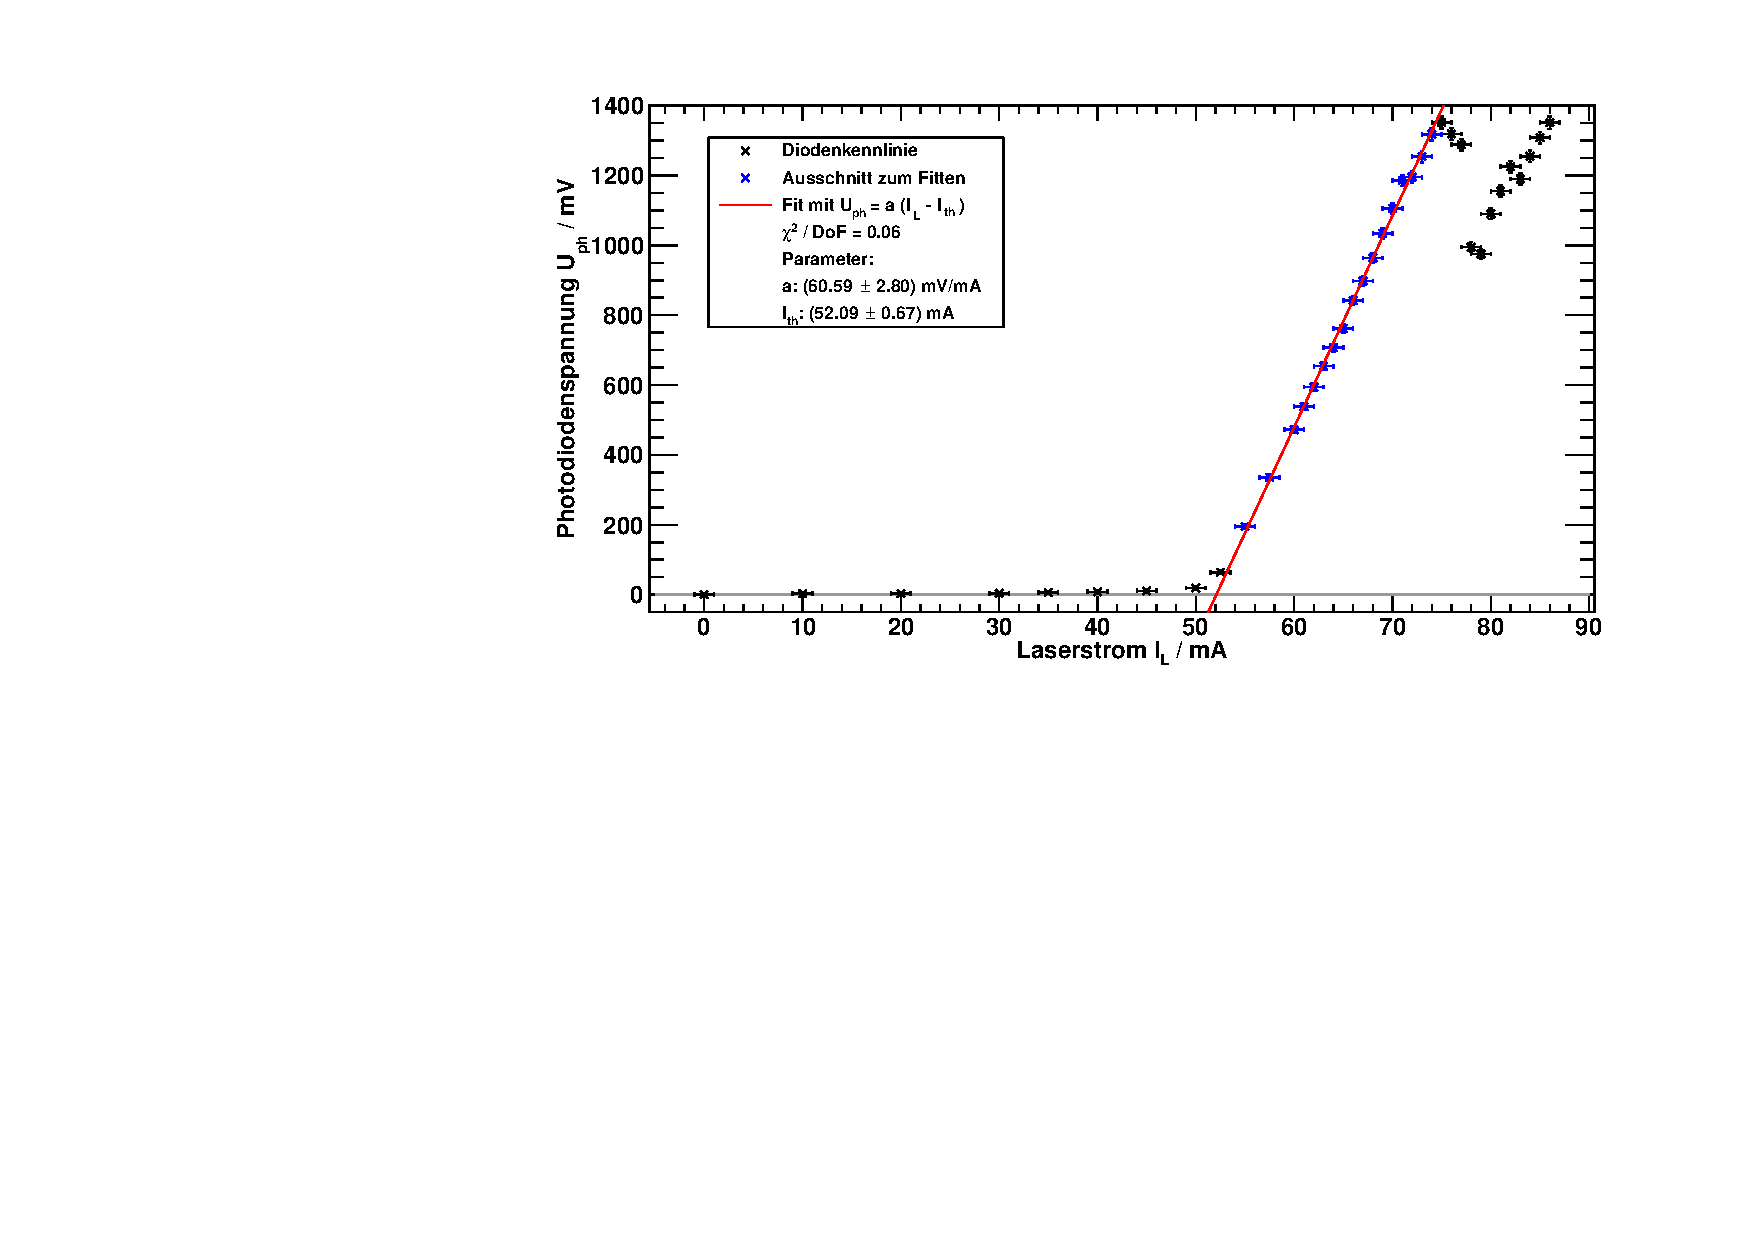
\includegraphics[width=\textwidth]{../img/part1/diodenkennlinie.pdf}
        \caption{$P$-$I$-Kennlinie der Laserdiode: Abhängigkeit der Spannung
        an der Photodiode vom Laserstrom $I_\text{L}$. Man erkennt den linearen Arbeitsbereich (gefitteter Teil),
        in dem ein modensprungfreier Betrieb möglich ist.}
        \label{img:Kennlinie}
    \end{center}
\end{figure}
\autoref{img:Kennlinie} zeigt die $P$-$I$-Kennlinie der Photodiode.
Als Fehler auf die Photodiodenspannung wurde ein Fehler von
\begin{equation}
    s_{U_{\text{ph}}}= 5\,\text{mV} + 0.01 \cdot U_{\text{ph}}
\end{equation}
angenommen.
Der Fehler auf den Strom $s_{I_{\text{L}}}$ beträgt ein Digit vom Lasernetzgerät:
\begin{equation}
    s_{I_{\text{L}}} = 0.1\,\text{mA} \ \, .
\end{equation}
Alle Messwerte wurden um den Spannungsoffset bei $I_{\text{L}}$=0\,mA verschoben.
Ein linearer Fit des modensprungfreien Laserbereichs zwischen 55\,mA und 71\,mA
liefert eine Laserschwelle $I_{\text{th}}$ von
\begin{equation}
    I_{\text{th}}=(52.01 \pm 0.13)\,\text{mA} \ \, .
\end{equation}
Interessant ist der Vergleich der $P$-$I$-Kennlinie mit dem Etalon-Transmissionsspektrum auf \autoref{img:etalon:fit}:
Aus der Amplitude der Modulationsspannung der Laserdiode und dem eingestellten Gleichanteil des Laserstroms
lässt sich der Laserstrom an den einzelnen Peaks bestimmen.
Dies wird hier kurz qualitativ gezeigt, ohne auf die Fehler einzugehen.

Der erste schwache Etalonpeak tritt bei einer Modulationsspannung von -0.26\,V auf, der Modensprung
bei einer Spannung von 0.22\,V.
Mit dem Konvertierungsfaktor des Lasernetzgeräts von 40\,mA/V und dem Gleichanteil des Laserstroms von 64.7\,mA
erhält man für den Laserstrom beim ersten Peak 54\,mA und beim Modensprung 74\,mA.
Dies entspricht fast exakt dem in der $P$-$I$-Kennlinie identifizierten Bereich
zwischen Laserschwelle und erstem Modensprung.




\section{Spektroskopie der Hyperfeinstruktur von Rubidium}
\subsection{Durchführung}
Bei der Messung des Hyperfein-Absorptionsspektrums befinden sich die beiden Linsen und
die Rubidiumzelle im Strahlengang.
Der Konstantanteil des Laserstroms, Modulationsamplitude und -frequenz
sind wie bei der Messung der Zeitabhängigkeit der Laserfrequenz (\autoref{sect:durchführung}).
Äußere Magnetfelder bleiben unkompensiert, weil die Zeeman-Aufspaltung der Hyperfeinstruktur im Erdmagnetfeld
mit der Linienbreite der Laserdiode nicht auflösbar ist.
Die Messung wird auf der steigenden und der fallenden Flanke der Modulationsspannung durchgeführt.


\subsection{Auswertung}
\subsubsection*{Frequenzeichung}
\subsubsection*{Hyperfeinstruktur-Übergänge}
\subsubsection*{Berechnung des Spektrums}
\subsubsection*{Vergleich mit den Literaturwerten}
Gerade sollte Steigung 1 und Achsenabschnitt 0 Ghz haben
\section{Doppelresonanzexperiment}
\subsection{Durchführung}
Für die Messung der Doppelresonanz ist das \textlambda/4-Plättchen in den Strahlengang eingesetzt.
Mit dem Linearpolarisator (im Strahlengang nach dem \textlambda/4-Plättchen) wird die
korrekte Win\-kel\-ein\-stel\-lung des \textlambda/4-Plättchens gefunden,
indem die Schwankungen der transmittierten Intensität
bei Drehung des Polarisators minimiert werden.
Der RF-Sender auf der Zelle wird verwendet, um ein hochfrequentes Wechselfeld in das Rubidiumgas einzustrahlen.
Die Messung der Frequenz erfolgt mit dem Frequenzzähler im Versuchsaufbau.
An Spule~2 wird mit dem \emph{instec function~generator} ein Sinussignal angelegt (siehe \autoref{img:dehmeltrf}),
das ein wechselndes Magnetfeld in Strahlrichtung erzeugt.
Mit der Photodiode wird die Intensität der Strahlung gemessen,
die durch die Rubidiumzelle gelangt.
Auf \autoref{img:dehmeltrf} ist zu sehen, dass zusätzlich zu den erwarteten vier Doppelresonanz-Peaks pro
Periode der Magnetfeldmodulation zwei weitere Peaks pro Periode auftreten.
Diese Peaks bleiben bestehen, wenn das RF-Feld ausgeschaltet wird (siehe \autoref{img:dehmelt}) und
werden durch die Umkehr des Magnetfelds verursacht. Dies wird genauer in \autoref{sect:dehmelt} untersucht.

Zur Messung der Doppelresonanz wird ein weiteres zeitlich konstantes Magnetfeld in Strahlrichtung erzeugt,
indem ein Gleichstrom durch Spule~1 geschickt wird.
Durch die Variation dieses Stroms kann die Position der Absorptionspeaks der Doppelresonanz eingestellt werden
(siehe \autoref{img:rfwrong} und \autoref{img:rfcorrect}).
Für zwei verschiedene Radiofrequenzen (494\,kHz und 900\,kHz) und
zwei verschiedene Laserströme (62.9\,mA und 63.2\,mA) werden so die acht 
Werte für die Stromstärken bestimmt, bei denen die Absorptionspeaks äquidistant sind.
Dazu ist es notwendig, die Polung des Spulenstroms durch Umstecken der Kabel umzukehren.

Die Amplitude des Sinussignals zur Magnetfeldmodulation beträgt bei der Messung 0.16\,V und
die Temperatur des Peltierelements 33.9$^\circ$C.
Außerdem werden an Spule~4 86\,mA Gleichstrom angelegt, um das vertikale Magnetfeld zu kompensieren.
Die Höhe des Stroms wird durch Maximierung der Signalintensität bestimmt.

\begin{figure}[H]
\begin{center}
  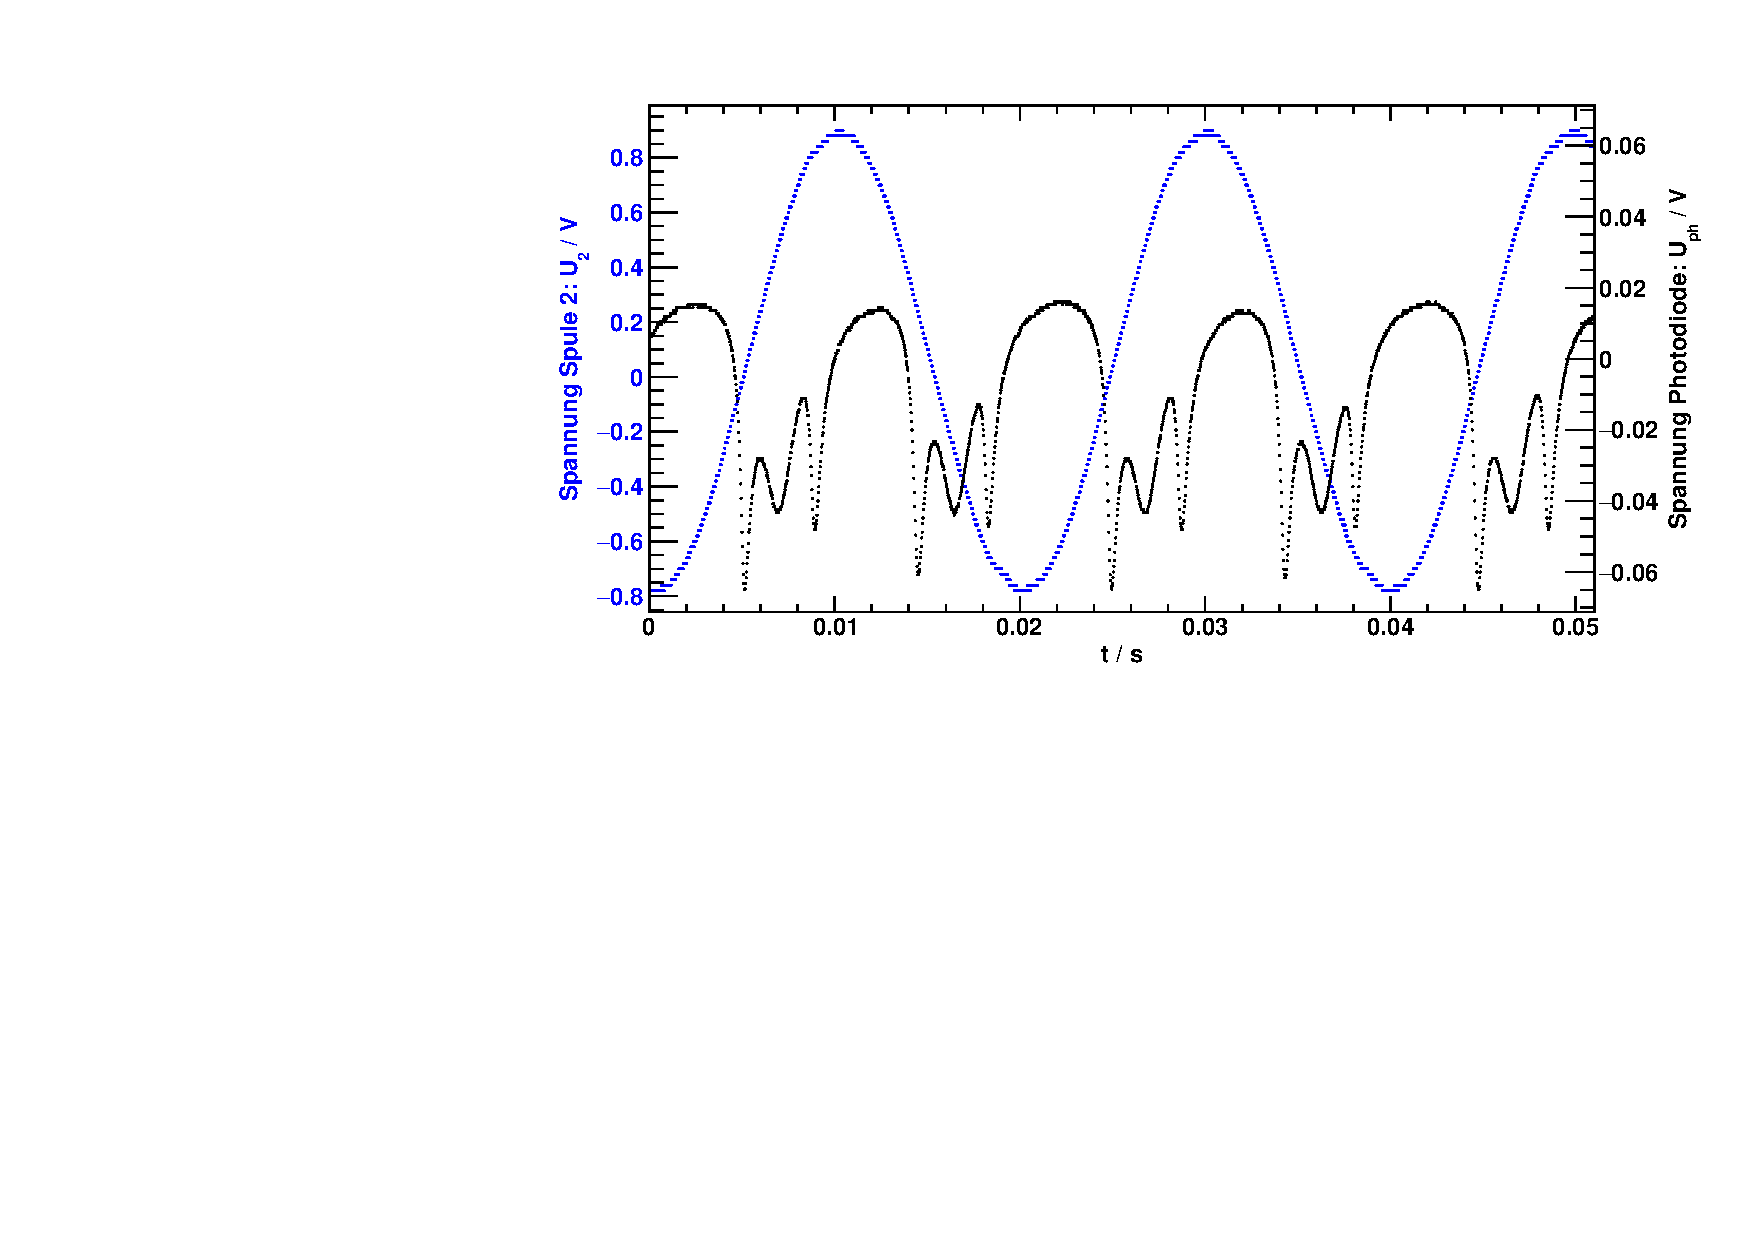
\includegraphics[width=\textwidth]{../img/part3/06.pdf}
  \caption{Starke Modulation des Magnetfelds in Strahlrichtung mit Spule~2 (blau).
   Im Photodiodensignal (schwarz) sind vier Doppelresonanz-Peaks sowie
   zwei Dehmelt-Peaks pro Modulationsperiode sichtbar.}
  \label{img:dehmeltrf}
\end{center}
\end{figure}

\begin{figure}[H]
\begin{center}
    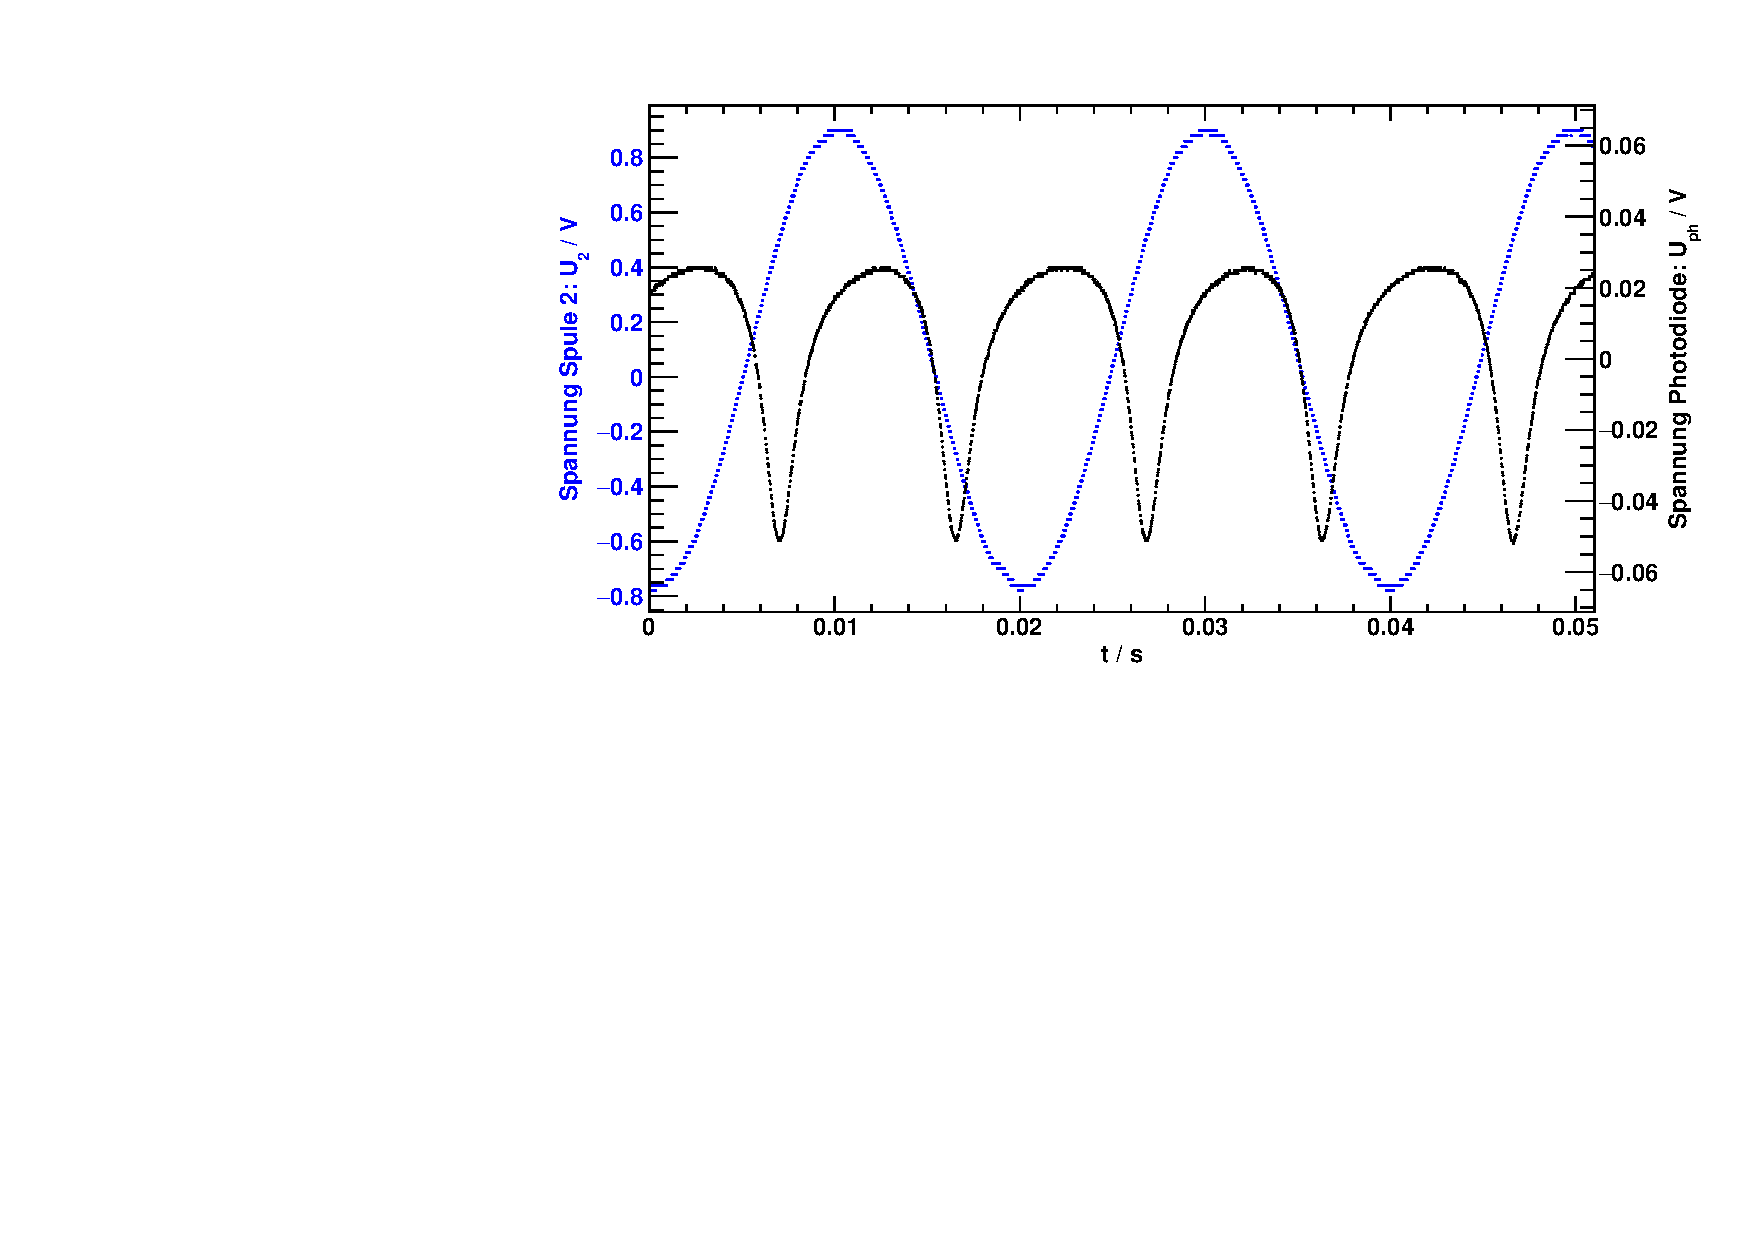
\includegraphics[width=\textwidth]{../img/part3/07.pdf}
    \caption{Gleiches Setup wie bei \autoref{img:dehmeltrf}, aber ohne RF-Signal.
    Die leicht asymmetrischen Dehmelt-Peaks sind weiterhin vorhanden.}
    \label{img:dehmelt}
\end{center}
\end{figure}

\begin{figure}[H]
\begin{center}
  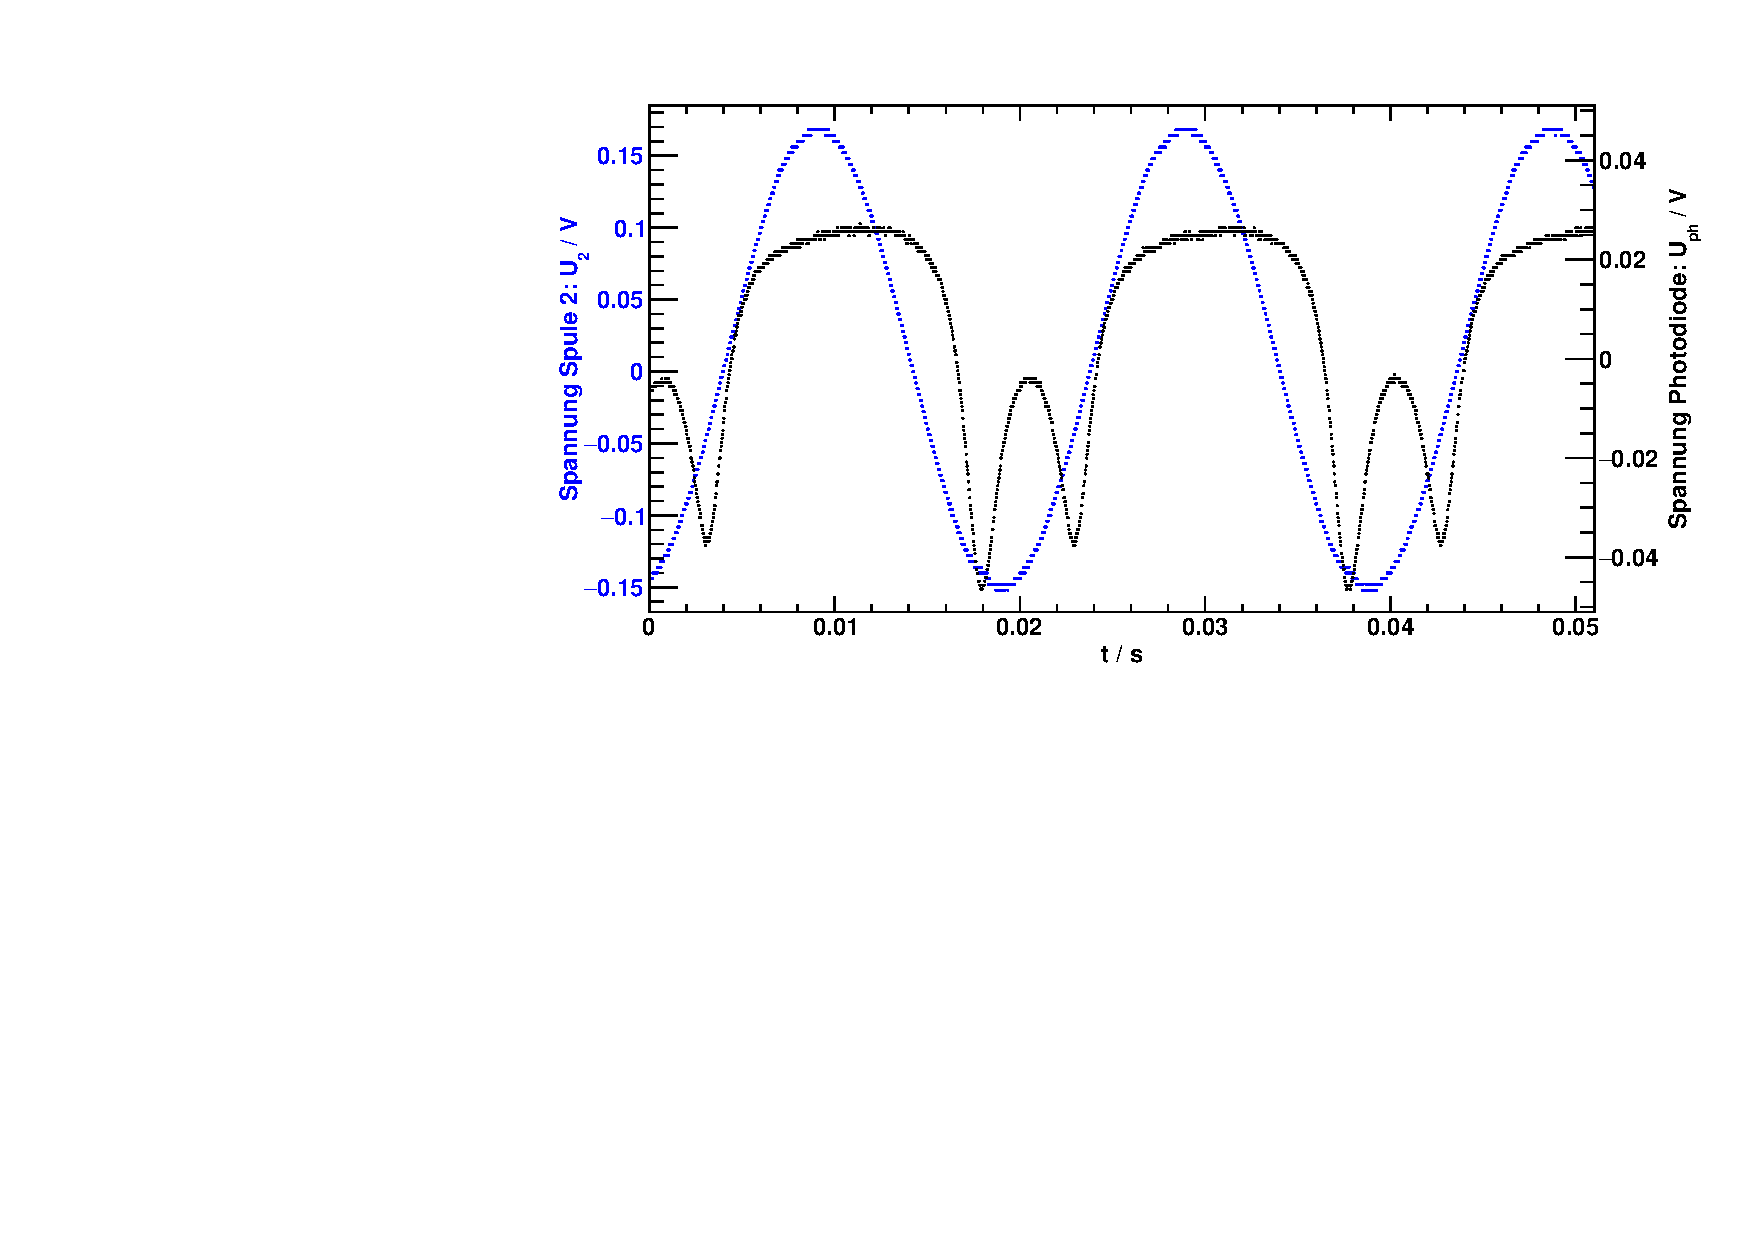
\includegraphics[width=\textwidth]{../img/part3/11.pdf}
  \caption{Doppelresonanz-Absorptionssignal bei kleiner Magnetfeldmodulation:
  Falsche Einstellung des Gleichstroms in Spule~1,
  die Absorptionen sind nicht äquidistant.}
  \label{img:rfwrong}
\end{center}
\end{figure}

\begin{figure}[H]
\begin{center}
  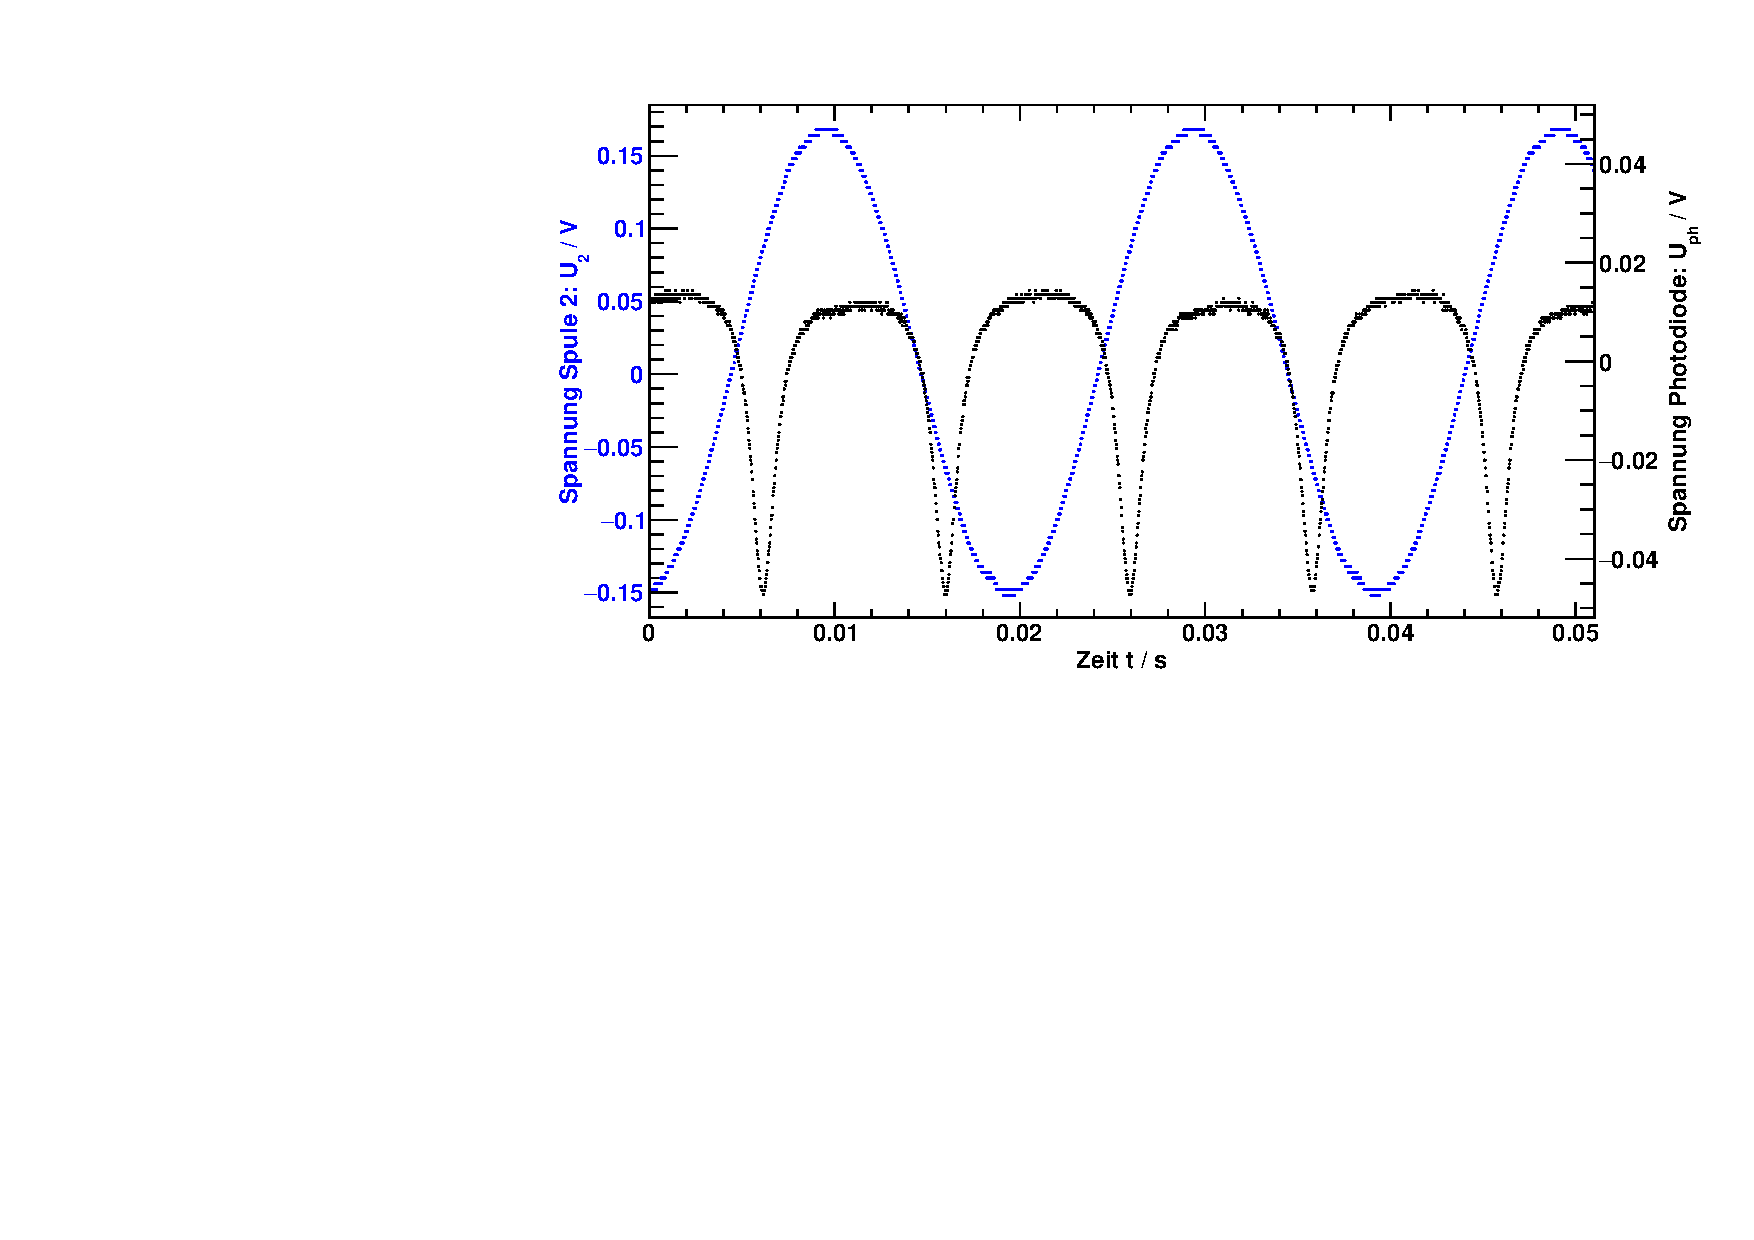
\includegraphics[width=\textwidth]{../img/part3/08.pdf}
  \caption{Doppelresonanz-Absorptionssignal bei kleiner Magnetfeldmodulation:
  Korrekte Einstellung des Gleichstroms in Spule~1,
  die Absorptionen sind daher äquidistant.}
  \label{img:rfcorrect}
\end{center}
\end{figure}

\subsection{Auswertung}
\label{sect:doppelresauswertung}
\subsubsection*{Berechnung des horizontalen und vertikalen Magnetfeldes und des Kernspins}
Die durch die Messung erhaltenen Ströme, welche durch Spule 1 ($I_1$ und bei Umpolung $I_1'$) fließen, sind in \autoref{tab:part3:data} 
aufgelistet. Der Strom $I_4$ von Spule 4 beträgt in allen Fällen
\begin{equation}
    I_4 = (86 \pm 3)\,\text{mA}
\end{equation}
Die Fehler auf den Laserstrom $I_L$ und die Frequenz $\nu$ des RF-Senders sind $s_{I_L} = 0.1$\,mA und $s_\nu=0.1$\,kHz. 
\begin{table}[H]
\caption{Messdaten des Doppelresonanzexperiments.}
\begin{center}
\begin{tabular}{|c|c|c|c|c|c|}
  \hline
  $I_\text{L}$ / mA & $\nu$ / kHz & $I_1$ / mA & $s_{I_1}$ / mA & $I_1'$ / mA & $s_{I_1'}$ / mA \\ \hline
  62.9 & 493.98 & 117 & 2 & 148 & 2 \\ \hline
  62.9 & 899.41 & 228 & 4 & 260 & 4 \\ \hline
  63.2 & 493.77 & 104 & 2 & 74 & 2 \\ \hline
  63.2 & 899.67 & 148 & 2 & 179 & 2 \\ \hline
\end{tabular}
\end{center}
\label{tab:part3:data}
\end{table}

Zuerst wird der Strom in den Spulen in das resultierende Magnetfeld mit den Faktoren $c_n$ in \autoref{tab:inductorItoB} umgerechnet.
\begin{equation}
    B_n = c_n \cdot I_n, \qquad s_{B} = B_n \cdot \sqrt{ \left( \frac{s_{I_n}}{I_n} \right)^2 + \left( \frac{s_{c_n}}{c_n} \right)^2 }
\end{equation}
Nun können das horizontale und vertikale Magnetfeld, $B_\text{hor}$ und $B_\text{ver}$, sowie der Kernspin von Rubidium bestimmt werden.
\begin{itemize}
    \item Zur Bestimmung des horizontalen Magnetfeldes $B_\text{hor}$ wird die Hälfte des Mittelwerts von $B_1$ und $B_1'$ berechnet:
    \begin{equation}
        B_\text{hor} = \frac{1}{2} \abs{B_1 - B_1'}, \qquad s_{B_\text{hor}} = \frac{1}{2} \sqrt{s_{B_1}^2 + s_{B_1'}^2}
    \end{equation}
    \item Die Stärke des vertikalen Magnetfeldes $B_\text{ver}$ ergibt sich direkt aus der Stärke von Spule 4:
    \begin{equation}
        B_\text{ver} = B_4
    \end{equation}
    \item Um den Kernspin zu berechnen, muss von dem gemessenen Magnetfeld $B_1$ bzw. $B_1'$ das horizontale Erdmagnetfeld addiert oder - je nach
    Polung - subtrahiert werden. Bildet man aus diesen zwei Werten den Mittelwert, so kürzt sich das Erdmagnetfeld heraus und es ergibt sich
    folgende Formel:
    \begin{equation}
        B_I = \frac{B_1 + B_1'}{2}, \qquad s_{B_I} = \frac{1}{2} \sqrt{s_{B_1}^2 + s_{B_1'}^2}
    \end{equation}
    Mit diesem Wert und der Frequenz $\nu$ des RF-Senders kann nun mit \autoref{eq:nuclearspin} der Kernspin $I$ bestimmt werden. %TODO Ref nuclear spin
    \begin{equation}
        I = \frac{\mu_B \cdot B_I}{h \cdot \nu} - \frac{1}{2}, \qquad s_I = \frac{\mu_B \cdot B_I}{h \cdot \nu} \sqrt{ \left( \frac{s_{B_I}}{B_I} \right)^2 + \left( \frac{s_\nu}{\nu} \right)^2}
    \end{equation}
\end{itemize}
\begin{table}[H]
\caption{Berechnete horizontale Komponenten des Erdmagnetfeldes und Kernspin von Rubidium für das Doppelresonanzexperiment bei verschiedenen Lasterströmen $I_\text{L}$ und RF-Sender Frequenzen $\nu$.}
\begin{center}
\begin{tabular}{|c|c|c|c|c|c|}
  \hline
  $I_\text{L}$ / mA & $\nu$ / kHz & $B_\text{hor}$ / \textmu T & $s_{B_\text{hor}}$ / \textmu T & $I$ & $s_I$ \\ \hline
  62.9 & 493.98 & 12.4 & 1.1 & 2.50 & 0.03 \\ \hline
  62.9 & 899.41 & 12.8 & 2.3 & 2.53 & 0.04 \\ \hline
  63.2 & 493.77 & 12.0 & 1.1 & 1.52 & 0.03 \\ \hline
  63.2 & 899.67 & 12.4 & 1.1 & 1.53 & 0.02 \\ \hline
\end{tabular}
\end{center}
\label{tab:part3:results}
\end{table}

\subsubsection*{Berechneten Werte und Vergleich mit Literatur- bzw. theoretischen Werten.}
In \autoref{tab:part3:results} sind die berechneten Werte des horizontalen Erdmagnetfeldes für die verschiedenen Laserströmen $I_L$ und 
RF-Sender-Frequenzen $\nu$ zusammengestellt. 
\begin{itemize}
    \item Das vertikale Erdmagnetfeld ergibt sich zu
    \begin{equation}
        B_\text{ver} = (40.94 \pm 1.43)\,\text{\textmu T}\ \, ,
    \end{equation}
    was sich mit dem Literaturwert\footnote{Die Literaturwerte des horizontalen und vertikalen Erdmagnetfeldes, sowie die theoretischen Werte der
    Kernspins wurden \cite{manual} entnommen.} innerhalb von einem 2-\textsigma-Intervall deckt.
    \begin{equation}
    \label{eq:litvalBver}
        B_\text{ver}^{\text{Lit.}} = 42.9\,\text{\textmu T}
    \end{equation}
    \item Aus den Werten und Fehlern des horizontalen Magnetfeldes wird das gewichtete Mittel gebildet. Man erhält
    \begin{equation}
        \bar{B}_\text{hor} = (12.3 \pm 0.6)\,\text{\textmu T}\ \, .
    \end{equation}
    Dies stimmt nicht mit dem Literaturwert überein.
    \begin{equation}
        B_\text{hor}^{\text{Lit.}} = 20.9\,\text{\textmu T}
    \end{equation}
    Grund dafür könnten Stromflüsse von elektrischen Geräten im Gebäude sein, die ein zusätzliches Magnetfeld erzeugen.
    \item Auch die beiden Werte des Kernspins für jedes Isotop werden gewichtet gemittelt:
    \begin{equation}
        I(\text{\rb{85}}) = 2.51 \pm 0.02, \qquad I(\text{\rb{87}}) = 1.53 \pm 0.16
    \end{equation}
    Der errechnete Wert des Kernspins für \rb{85} stimmt innerhalb der Fehlergrenzen mit dem theoretischen Wert überein, 
    für \rb{87} im 2-\textsigma-Intervall.
    \begin{equation}
        I(\text{\rb{85}})^\text{theo.} = 2.5, \qquad I(\text{\rb{87}})^\text{theo.} = 1.5
    \end{equation}
\end{itemize}
\section{Spinpräzession im Erdmagnetfeld}
\subsection{Durchführung}
Die Bestimmung der Spinpräzession im vertikalen Erdmagnetfeld erfolgt folgendermaßen:
Das \textlambda/4-Plättchen im Strahlengang erzeugt zirkular polarisiertes Licht,
durch das die Rubidiumatome im Magnetfeld optisch gepumpt werden.
Das Magnetfeld wird von Spule~5 erzeugt, ihre Stromversorgung erfolgt vom \emph{instec function~generator}.
Der Funktionsgenerator erzeugt ein Rechtecksignal mit einer Spitze-zu-Spitze-Amplitude von 260\,mV und
einem Offset von 130\,mV, sodass das Magnetfeld periodisch an- und ausgeschaltet wird.
Um das Erdmagnetfeld in Strahlrichtung zu kompensieren,
wird ein Strom von $I_1$=17\,mA durch Spule~1 geschickt.
Die Temperatur des Peltierelements beträgt bei den Messungen 33.9$^\circ$C.
Es werden zuerst zwei Messreihen durchgeführt, um die beiden Rubidiumisotope zu untersuchen:
Mit 63.7\,mA Laserstrom (Pumpen von \rb{85}) und mit 64.1\,mA (\rb{87}).
Während einer Messreihe wird der Strom durch Spule~4 zwischen 0\,mA und 100\,mA variiert und
so die Vertikalkomponente des Magnetfelds beeinflusst
(eine Kompensation des vertikalen Erdmagnetfeldes findet bei ca. 90\,mA statt).
Das Transmissionssignal der Messzelle wird mit dem Oszilloskop gemessen und
es findet eine Heizung mit dem Föhn statt.

Nach Durchführung der ersten beiden Messungen wurde festgestellt,
dass mit der Variation des Stroms durch Spule~4 keine vollständige Kompensation des Magnetfelds möglich ist.
(Eine vollständige Kompensation würde sich darin zeigen,
dass die Frequenz der Spinpräzession sehr groß wird und keine Präzession mehr messbar ist).
Dies wurde auf die Anwesenheit der Horizontalkomponente des Erdmagnetfeldes
senkrecht zum Strahlengang zurückgeführt, da der Messaufbau nicht parallel zum Horizontalanteil des
Erdmagnetfelds ausgerichtet ist und durch Spule~1 nur ein Magnetfeld parallel zum Strahlengang kompensiert wird.

Aus dem Anteil des Magnetfelds, das bei den ersten beiden Messreihen nicht kompensierbar war
(dieser Anteil wurde mit einem Modell bestimmt, das an die Messdaten angepasst wurde),
konnte die Abweichung des Messaufbaus von der Nordausrichtung vorhergesagt werden.
Der Messaufbau wurde um den so bestimmten Winkel gedreht und eine weitere Messreihe an \rb{85} durchgeführt,
um eine vollständige Magnetfeldkompensation und ein Verschwinden der Spinpräzession zu erreichen.
Zusätzlich wurde bei einem Strom von 90\,mA durch Spule~4 die Winkelabhängigkeit der Präzessionsfrequenz untersucht.


\subsection{Auswertung}
\begin{figure}[H]
\begin{center}
  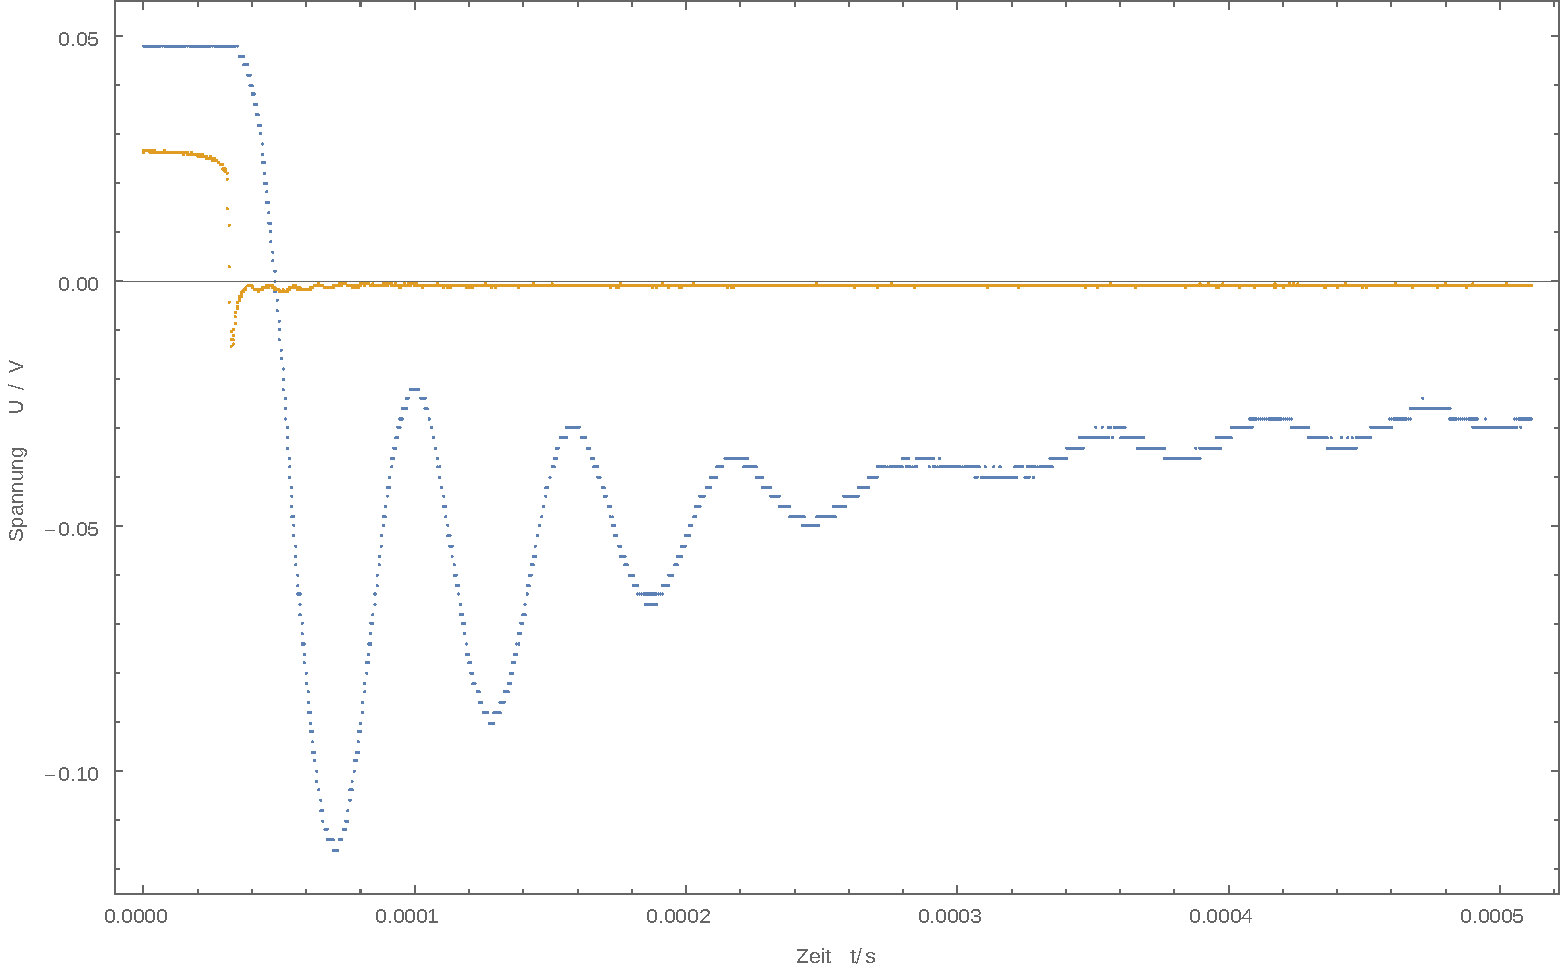
\includegraphics[width=\textwidth]{../img/part4/dummyExampleSpinpr.pdf}
  \caption{Spinpräzession des Rubidiumensembles, sichtbar in der Transmissionsoszillation der Messzelle.}
  \label{img:spp:expl}
\end{center}
\end{figure} 

\autoref{img:spp:expl} zeigt eines der gemessen Spinpräzessionssignale.
Zur Bestimmung der Präzessionsperiodendauer $T$ wurden die Zeitkoordinaten $t_1$ und $t_2$
von zwei möglichst weit voneinander entfernten Maxima per Hand abgelesen und durch
die Zahl $n$ der dazwischenliegenden Perioden geteilt:
\begin{equation}
  T=\frac{t_2-t_1}{n}=f^{-1}, \qquad s_f = n \frac{\sqrt{s_{t_2}^2 + s_{t_1}^2}}{ \left( t_2 -t_1 \right)^2 }
\end{equation}
Die Präzessionsfrequenz ist $f$ bezeichnet.
Der relative Fehler auf die abgelesenen Zeiten wurde auf $\frac{s_{t_i}}{t_i}=0.01$ abgeschätzt,
$n$ ist nicht fehlerbehaftet.

Aus dem Strom durch Spule~4 wurde mit \autoref{tab:inductorItoB} das erzeugte vertikale Magnetfeld
$B_\text{S,v}$ berechnet. Der Fehler auf den Strom beträgt $s_{I_4}=1$\,mA.

Die Abhängigkeit der Präzessionsfrequenz $f$ vom zusätzlichen Vertikalfeld $B_\text{S,v}$ ist auf
\autoref{img:spp:SPPRb85} gezeigt.
Ein erster Fit erfolgt mit
\begin{equation}
  f_1(B_\text{S,v})=\alpha \cdot |B_\text{E,v}-B_\text{S,v}| \ \, ,
\end{equation}
wobei $B_\text{E,v}$ die Vertikalkomponente des Erdmagnetfelds bezeichnet und
$\alpha_1$ eine Proportionalitätskonstante.
Es ist deutlich erkennbar, dass das lineare Modell die Messwerte nur beschreiben kann,
wenn sich die Richtung des effektiven Vertikalfeldes
$B_\text{E,v} \text{\,-\,} B_\text{S,v}$ in der Messreihe nicht umdreht.

\begin{figure}[H]
\begin{center}
  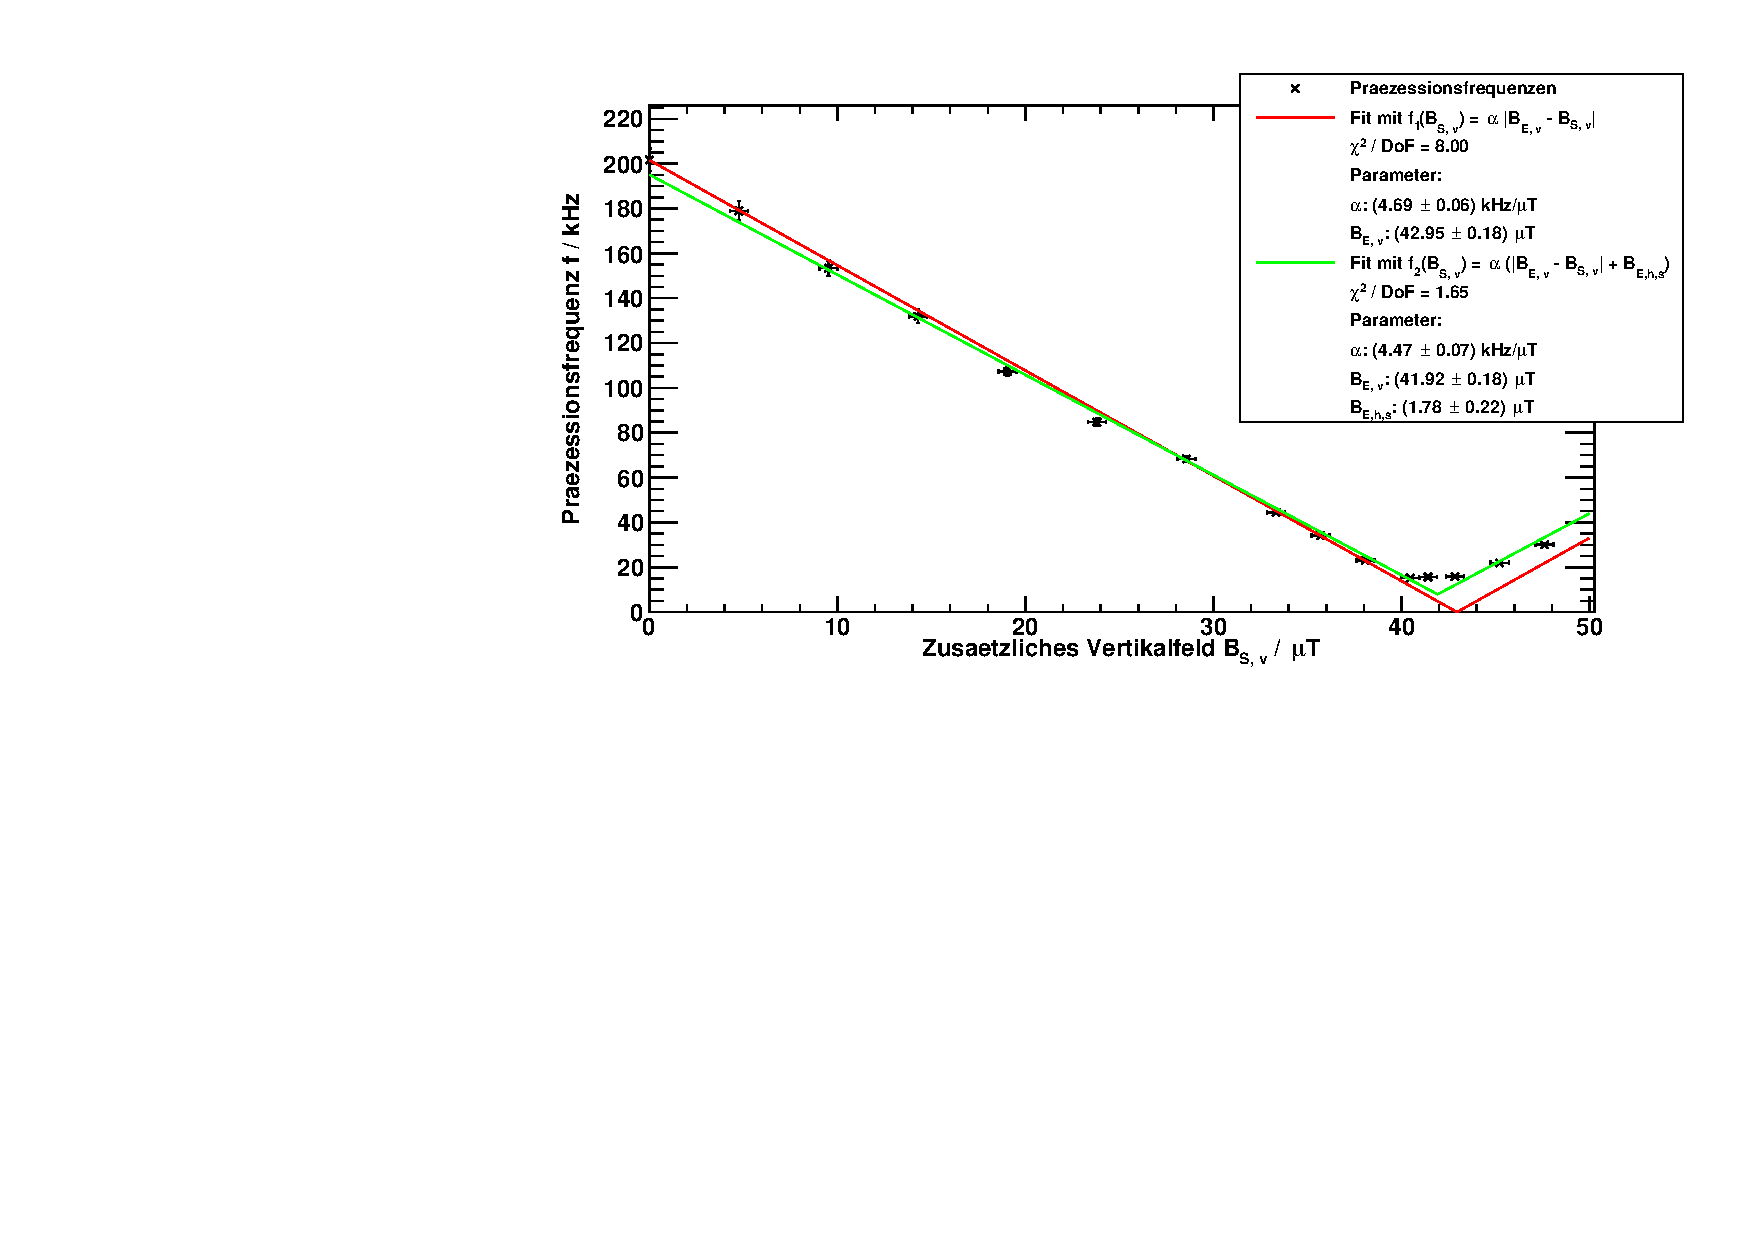
\includegraphics[width=\textwidth]{../img/part4/Rb85.pdf}
  \caption{Spinpräzessionsfrequenz $f$ von \rb{85} in Abhängigkeit
  vom zusätzlichen vertikalen Magnetfeld $B_\text{S,v}$, das dem Erdmagnetfeld überlagert ist.
  Der Fit erfolgt mit einem einfachen Modell sowie unter Berücksichtigung des
  nichtkompensierten Erdmagnetfelds~$B_\text{E,h,s}$.}
  \label{img:spp:SPPRb85}
\end{center}
\end{figure} 

Aus diesem Grund wird ein modifiziertes Modell verwendet, das der Tatsache Rechnung trägt,
dass der Horizontalanteil des Erdmagnetfelds senkrecht zum Strahl $B_\text{E,h,s}$
während der Messung unkompensiert bleibt:
\begin{equation}
  f_2(B_\text{S,v})=\alpha \cdot (|B_\text{E,v}-B_\text{S,v}| + B_\text{E,h,s}) \ \, .
\end{equation}
Dieses Modell eignet sich zur Beschreibung der Messdaten.

Die Auswertung erfolgt analog für das Isotop \rb{87} (\autoref{img:spp:SPPRb87}).
In \autoref{tab:spp:fitres} sind die Ergebnisse der aller vier Fits aufgeführt.

\begin{figure}[H]
\begin{center}
  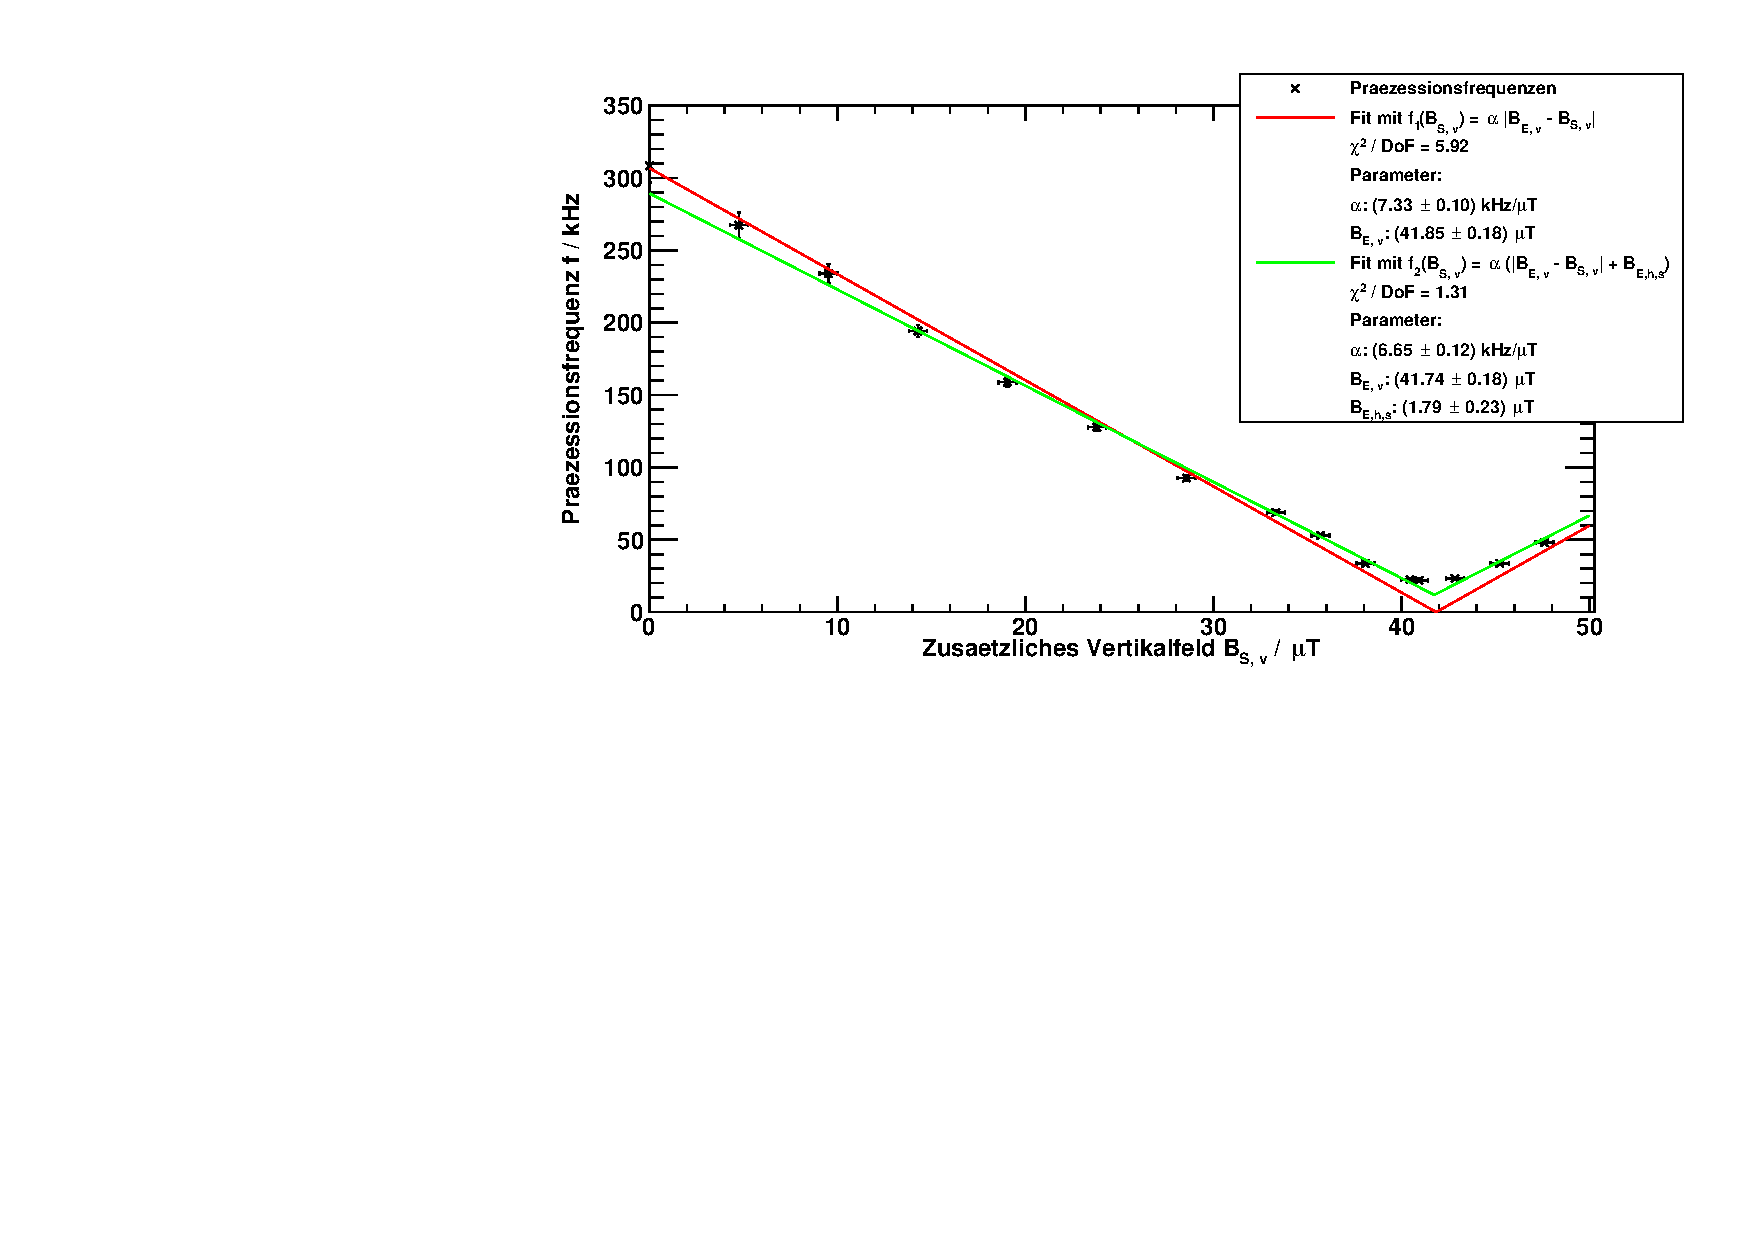
\includegraphics[width=\textwidth]{../img/part4/Rb87.pdf}
  \caption{Spinpräzessionsfrequenz $f$ von \rb{87} in Abhängigkeit
  vom zusätzlichen vertikalen Magnetfeld $B_\text{S,v}$.}
  \label{img:spp:SPPRb87}
\end{center}
\end{figure} 


\begin{table}[H]
\caption{Ergebnisse der Fits der Präzessionsfrequenzen
für die Komponenten des Erdmagnetfeldes und die Proportionalitätskonstante $\alpha$.}
\begin{center}
\begin{tabular}{|c|c|c|c|c|}
  \hline	
	Fit						& $B_\text{E,v}$ / \textmu T	& $B_\text{E,h,s}$ / \textmu T	& $\alpha$ / (ms \textmu T)$^{-1}$	& $\alpha^\text{theo}$ / (ms \textmu T)$^{-1}$ \\ \hline
  \rb{85}: \emph{Modell 1}	& 38.9$\,\pm\,$0.4				& $-$ 							& 5.7$\,\pm\,$0.5 					& 4.665											\\ \hline
  \rb{85}: \emph{Modell 2}	& 38.61$\,\pm\,$0.17			& 2.3$\,\pm\,$0.3				& 4.5$\,\pm\,$0.2 					& 4.665											\\ \hline
  \rb{87}: \emph{Modell 1}	& 38.7$\,\pm\,$0.4				& $-$ 							& 8.6$\,\pm\,$0.8 					& 6.998											\\ \hline
  \rb{87}: \emph{Modell 2}	& 38.44$\,\pm\,$0.12			& 2.09$\,\pm\,$0.19				& 6.9$\,\pm\,$0.2 					& 6.998											\\ \hline
  
\end{tabular}
\end{center}
\label{tab:spp:fitres}
\end{table}
%TODO Einheit alpha
%TODO richtige fitergebnisse

Die Ergebnisse für das vertikale Erdmagnetfeld stimmen nicht mit dem Literaturwert (\autoref{eq:litvalBver}) überein.
Die Ursache dafür könnten Magnetfelder von elektrischen Geräten im Gebäude sein,
die dem Erdmagnetfeld überlagert sind.

Man erkennt, dass der Fehler auf die Proportionalitätskonstante $\alpha$ bei den einfachen Modellen sehr groß ist.
Der theoretische Wert liegt ungefähr zwei Standardabweichungen vom experimentellen Wert entfernt.
Das komplexere Modell liefert $\alpha$ mit einem viel kleineren Fehler,
außerdem liegt hier der theoretische Wert innerhalb
einer Standardabweichung.
%%TODO stimmt das noch?

Zusätzlich erhält man im zweiten Modell einen Wert für die unkompensierte Horizontalkomponente des Erdmagnetfelds $B_\text{E,h,s}$.
Da in \autoref{sect:doppelresauswertung} der Wert für die Horizontalkomponente des Erdmagnetfelds in
Strahlrichtung ($\bar{B}_\text{hor}$ = (12.3$\,\pm\,$0.6)\,\textmu T) bestimmt wurde,
lässt sich nun mit einfachen trigonometrischen Überlegungen der Winkel $\varphi$ berechnen,
um der Strahlengang von Norden abweicht:
\begin{equation}
  \varphi = \text{Arcsin}\left( \frac{B_\text{E,h,s}}{\bar{B}_\text{hor}} \right)
\end{equation}
Man erhält damit für die beiden Messreihen
\begin{equation}
  \varphi_{85} = (11.6 \pm 1.3)^\circ \qquad \text{und} \qquad \varphi_{87} = (9.8 \pm 1.0)^\circ \ \, .
\end{equation}
%%TODO stimmt das noch?

Der Messaufbau wurde also um 10$^\circ$ gegen den Uhrzeigersinn gedreht
(für die Drehrichtung entscheiden wir uns nach einem Blick auf eine Landkarte)
und die Messung an \rb{85} erneut durchgeführt.
\autoref{img:spp:SPPRb87gedr} zeigt die Messung und den Fit mit dem einfachen Modell,
das diese Messdaten jetzt geeignet beschreibt.
Die obige Verwendung des erweiterten Modells lieferte also hier eine korrekte Vorhersage.

\begin{figure}[H]
\begin{center}
  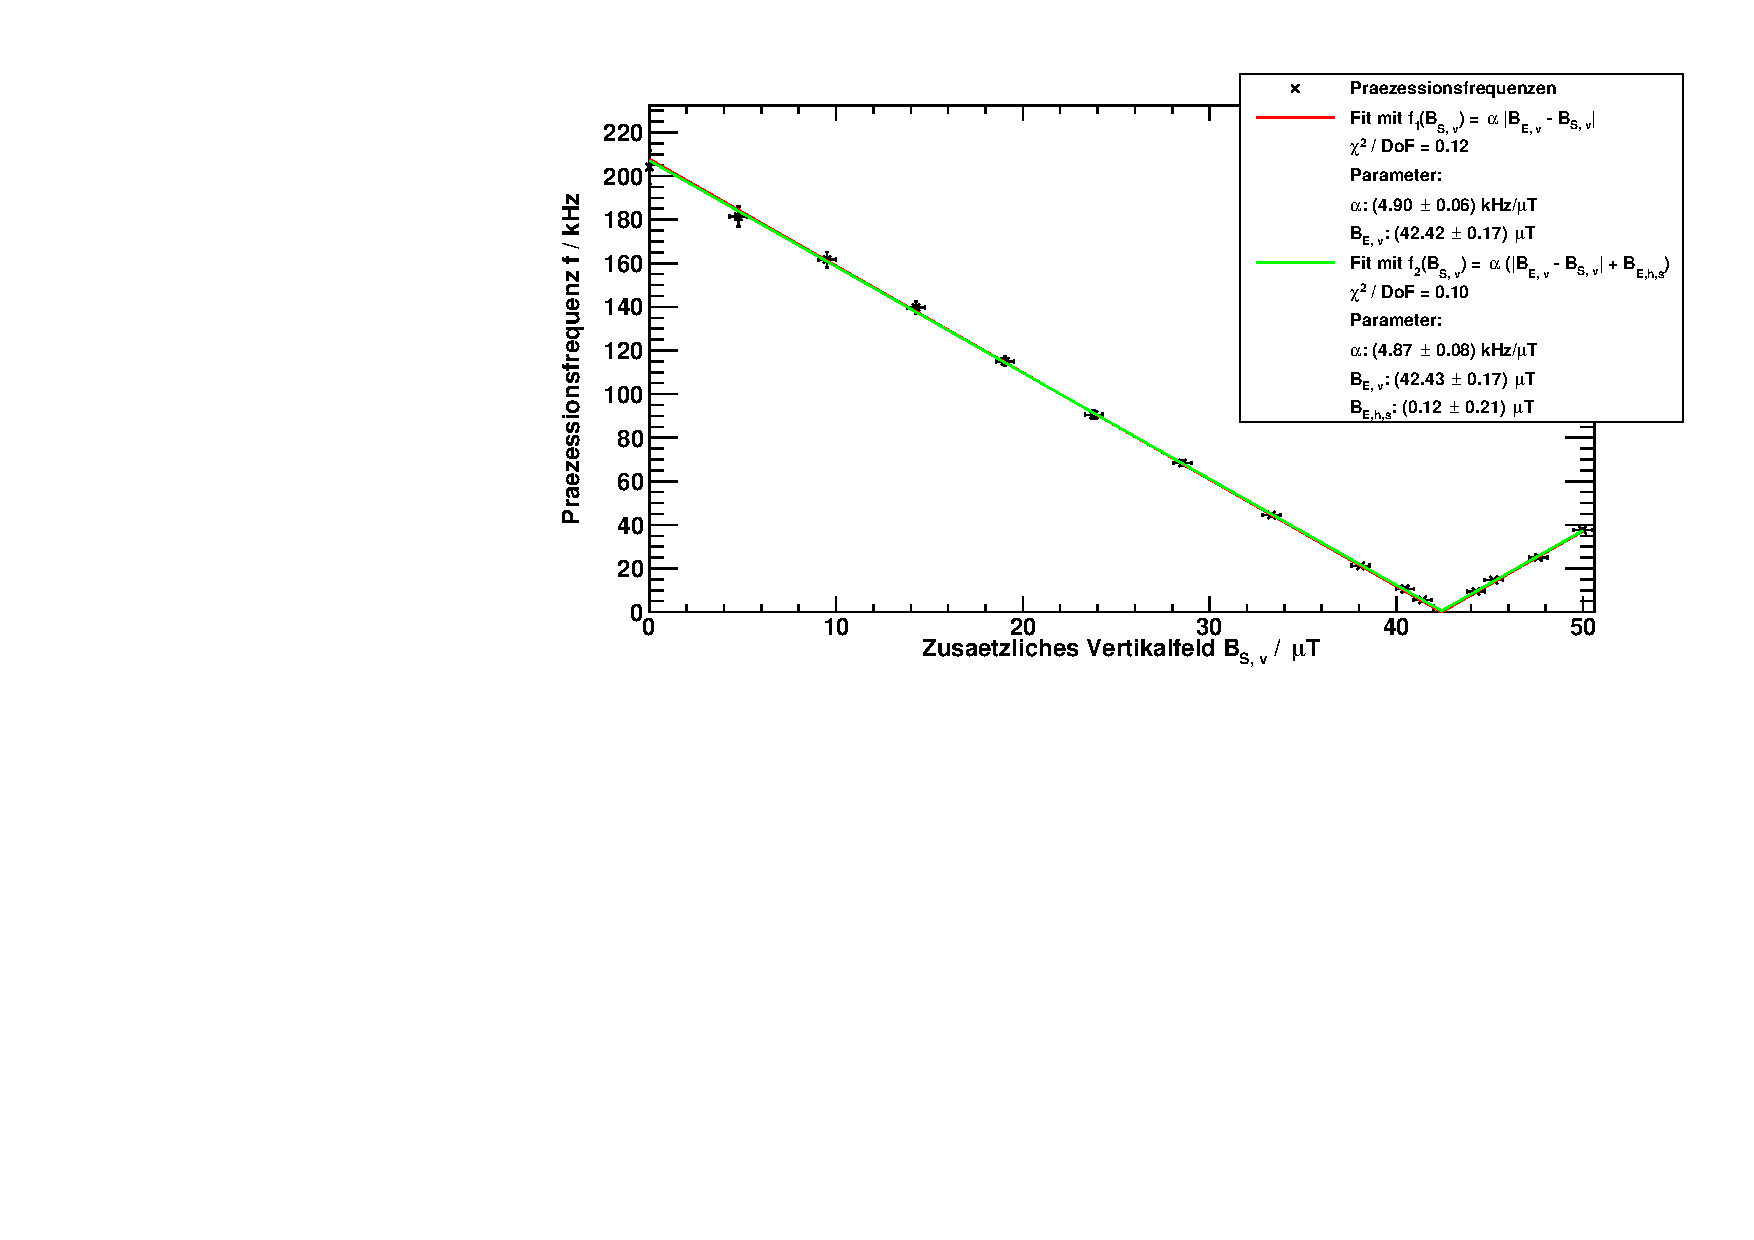
\includegraphics[width=\textwidth]{../img/part4/Rb85_gedreht.pdf}
  \caption{Spinpräzessionsfrequenz $f$ von \rb{85} in Abhängigkeit
  vom zusätzlichen vertikalen Magnetfeld $B_\text{S,v}$
  nach Drehung des Messaufbaus um 10$^\circ$ gegen den Uhrzeigersinn.}
  \label{img:spp:SPPRb87gedr}
\end{center}
\end{figure} 

Als Fitparameter erhält man
\begin{equation}
  B_\text{E,v} = (39.09\,\pm\,0.02)\,\text{\textmu T} \qquad \text{und} \qquad \alpha = (5.42\,\pm\,0.03)\,\text{ms}^{-1} \text{\textmu T}^{-1}
\end{equation}
Der Wert für das vertikale Erdmagnetfeld stimmt aus dem oben erwähnten Grund nicht mit dem Literaturwert überein.
Für die starke Abweichung des Parameters $\alpha$ vom theoretischen Wert $\alpha^\text{theo}$\,=\,4.665\,ms$^{-1}$\textmu T$^{-1}$ haben wir keine Erklärung.\\

Eine weitere Untersuchung der Horizontalkomponente erfolgte mit einer Untersuchung der Winkelabhängigkeit
der Präzessionsfrequenz.
Für sie gilt
\begin{equation}
  f(\varphi) = \alpha \cdot B_\text{E,h,p} \cdot |\sin(\varphi)| \ \, ,  %TODO Parameter für Winkeloffset, sollte verschwinden
\end{equation}
mit der Horizontalkomponente $B_\text{E,h,p}$ des Erdmagnetfelds in Strahlrichtung.
\autoref{img:spp:Winkelabhängigkeit} zeigt die Messergebnisse und den Fit mit obiger Gleichung.
Leider erlaubten die Abmessungen des Aufbaus eine Messung nur im Bereich von -10$^\circ$ bis 10$^\circ$,
so dass für den Sinus auch die Kleinwinkelnäherung verwendet werden könnte.

\begin{figure}[H]
\begin{center}
  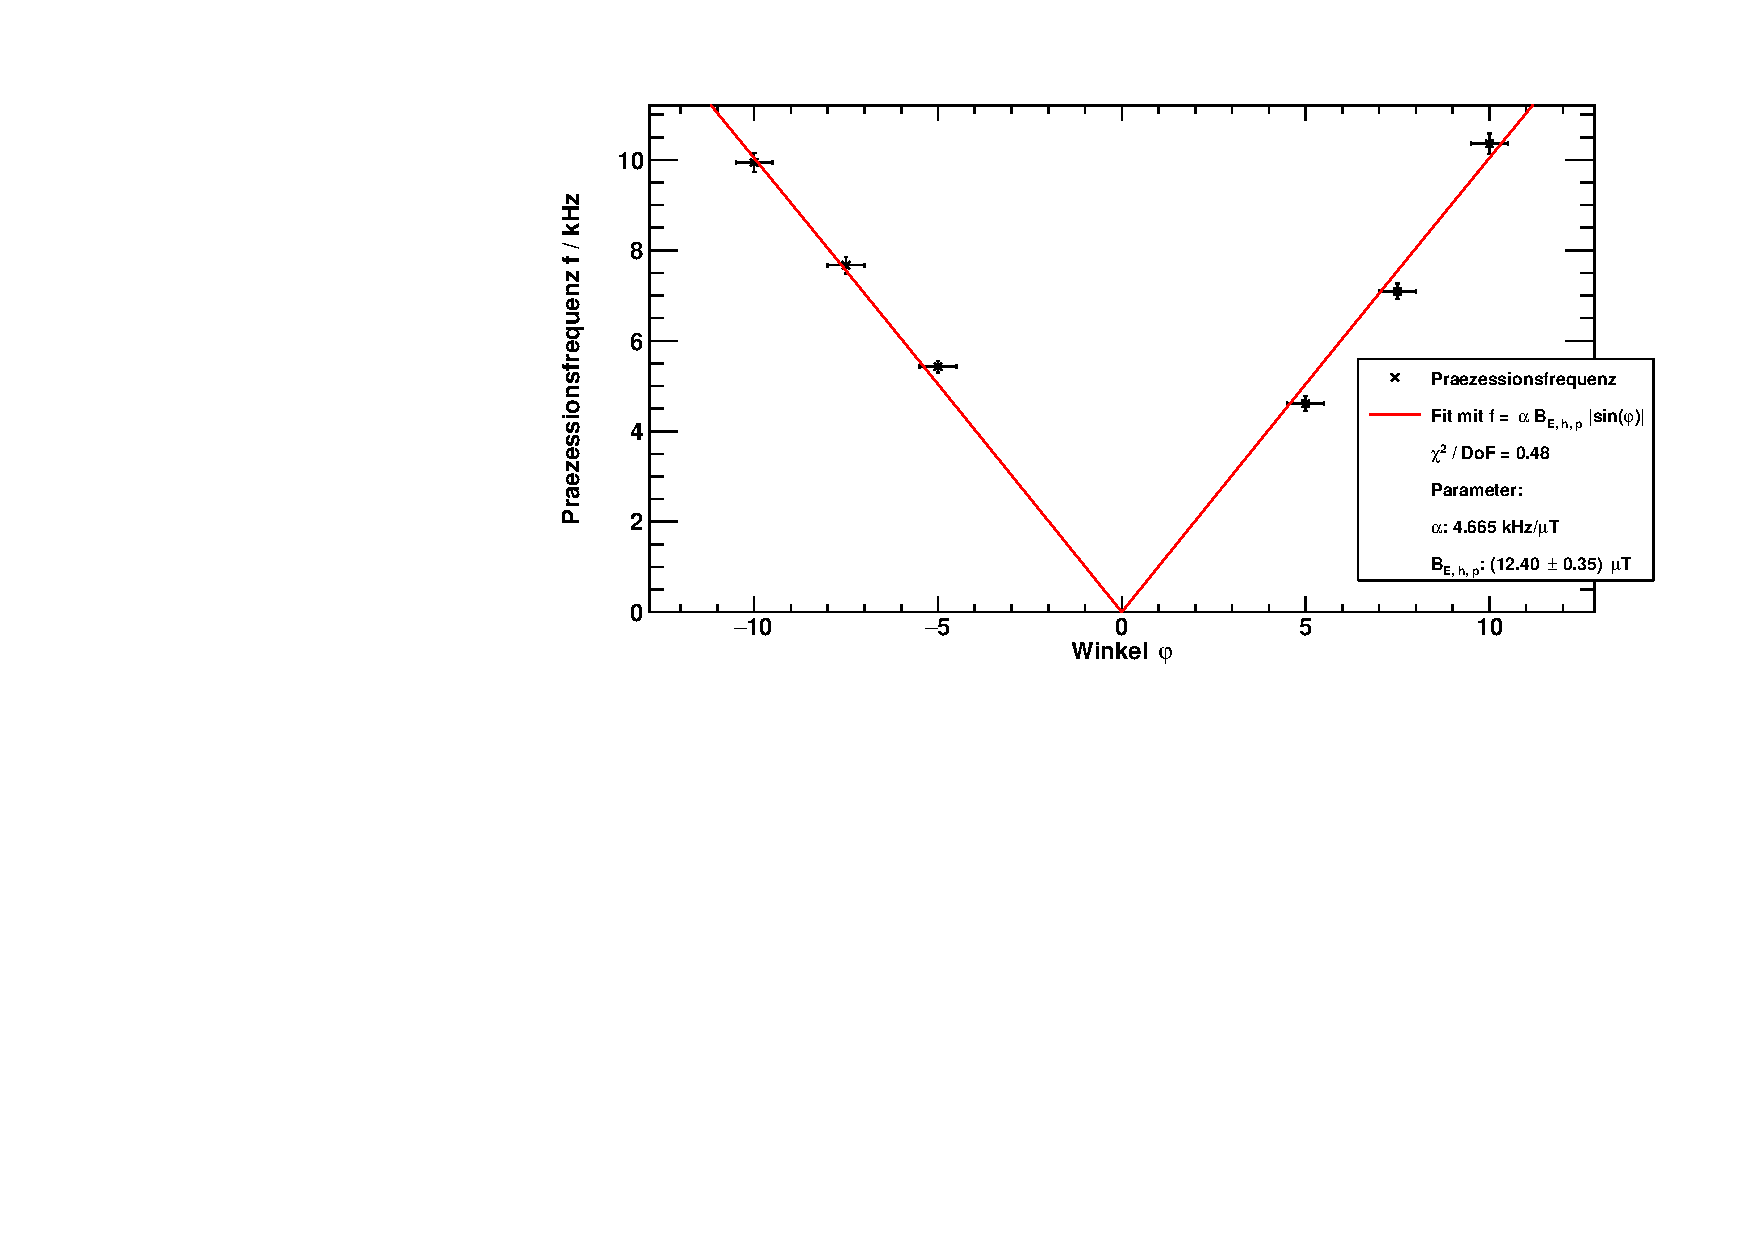
\includegraphics[width=\textwidth]{../img/part4/winkel.pdf}
  \caption{Abhängigkeit der Spinpräzessionsfrequenz $f$ von der Ausrichtung des Messaufbaus im Erdmagnetfeld.}
  \label{img:spp:Winkelabhängigkeit}
\end{center}
\end{figure} 

Die Horizontalkomponente des Erdmagnetfelds beträgt laut den oben gewonnenen Messdaten
\begin{equation}
  B_\text{E,h,p} = \sqrt{\bar{B}_\text{hor}^2+B_\text{E,h,s}^2}=(12.5 \pm 0.2)\,\text{\textmu T} \ \, .
\end{equation}
%TODO richtige Werte
Damit erhält man aus der Steigung der Fitgeraden $a$ für die Proportionalitätskonstante
\begin{equation}
  \alpha = \frac{a}{B_\text{E,h,p}} = (4.56\pm0.02)\,\text{ms}^{-1} \text{\textmu T}^{-1} \ \, .
\end{equation}
%TODO richtige Werte
Dieser Wert stimmt..
%TODO vgl Litval
\section{Messung der Spin-Relaxationszeit nach Dehmelt}
\label{sect:dehmelt}
\subsection{Durchführung}
Bei dieser Methode der Bestimmung der Spin-Relaxationszeit wird die Tatsache ausgenutzt,
dass bei Beleuchtung des Ensembles der Rubidiumatome durch \textsigma$^+$-Licht
zwei konkurrierende Prozesse vorliegen, die den Orientierungsprozess der Spins und damit
die Lichttransmission durch das Ensemble beeinflussen:
Zum einen findet eine Polarisation durch den Pumpprozess statt,
zu anderen eine Depolarisation (Relaxation) durch Stöße der Gasatome mit dem Glaskolben.
Eine Variation der Stärke des Pumpprozesses durch Veränderung der Intensität des Laserlichts
erlaubt einen Rückschluss auf den konstantbleibenden Anteil der Relaxationsrate.

Während der Messung befinden sich die beiden Linsen und das \textlambda/4-Plättchen im Strahlengang,
sowie optional ein Neutraldichtefilter.
Das vertikale Erdmagnetfeld wird mit einem Strom von 93\,mA durch Spule~4 kompensiert.
Spule~3 erzeugt ein magnetisches Wechselfeld in Richtung des Laserstrahls,
das zweimal pro Periode eine Neuorientierung des Ensembles verursacht.
Verwendet wird dazu der \emph{Instec function~generator},
die Frequenz des Rechtecksignals beträgt 50\,Hz und die Amplitude (Spitze-Spitze) 0.1\,V.

Das Absorptionssignal der Zelle wird am Oszilloskop erst mit 100\% Beleuchtungsintensität gemessen
und anschließend mit sieben verschiedenen Intensitäten (zwischen 2\% und 40\%),
die durch unterschiedliche Abschwächungen mit ND-Filtern im Strahlengang erreicht werden.

Die Temperatur des Lasers beträgt bei der Messung 34.0$^\circ$C, der Laserstrom 65.5\,mA
(so~dass auf den beiden kurzwelligen Hyperfeinlinien von \rb{85} gepumpt wird).







\subsubsection*{Kalibrierung der Neutraldichtefilter}
Um die Stärke der verschiedenen Neutraldichtefilter festzustellen,
wird eine Kalibrierung mit Laser und Photodiode durchgeführt.
Die Temperatur des Lasers beträgt dabei 34.0$^\circ$C, der Laserstrom 52.0\,mA.
Die Spannung an der Photodiode wird ohne Filter gemessen und anschließend für zehn verschiedene Graufilter
mit nominellen Transmissivitäten von 0.001\% bis 50\%.
Ein weiterer Messpunkt wird mit ausgeschaltetem Laser aufgenommen.


\subsection{Auswertung}

\subsubsection*{Kalibrierung der Neutraldichtefilter}

\autoref{tab:deh:dnfilter} zeigt die Ergebnisse der Kalibrierung der Neutraldichtefilter:
Die Messwerte weichen stark von den nominellen Werten ab.
Zur Berechnung der transmittierten Intensität $I_\text{t}$ wird
die an der Photodiode gemessene Spannung $U_{\text{ph}}$
durch die Spannung bei 100\% Intensität $U_{100}$ geteilt.
Beide Spannungen werden um die Offsetspannung $U_{0}$ (Messung bei ausgeschaltetem Laser) korrigiert:
\begin{equation}
  I_\text{t}=\frac{U_{\text{ph}}+U_{0}}{U_{100}+U_{0}}
\end{equation}
Die Berechnung des Fehlers erfolgt mit Gaußscher Fehlerfortpflanzung.

Für die Bestimmung der Relaxationszeit werden nur die ersten sieben Filter verwendet,
da bei den Übrigen die Intensität der Transmission nicht für eine Messung ausreicht.


%TODO Tabelle ND Filter
TABELLE ND Filter


STÄRKE		NOM. INTENS 	gem. Spannung		Gem. intens 	error gem. intens

ohne 

0.3	 			50\%			300\,mV				30\%


\subsubsection*{Fit der Transmissionssignale}
\autoref{img:deh:trans3} zeigt die Spannung der Photodiode $U$, die am Oszilloskop gemessen wurde.
Sie ist proportional zur transmittierten Lichtintensität.
Der Fit erfolgt mit einer e-Funktion:
\begin{equation}
  U(t)=a - b \cdot e^{-\frac{t}{\tau}}
\end{equation}
Der Parameter $a$ beschreibt die Transmission im Gleichgewicht, $b$ die Amplitude der
Transmissionsänderung direkt nach Umkehrung des Magnetfelds und $\tau$ die gesuchte Orientierungzeit des Ensembles.


Abb Beispiel von Transmissionssignal
 %TODO Abb von dritter Dehlemt-Transmission
 

In \autoref{tab:deh:fitres} sind die Ergebnisse aller acht Fits an die Transmissionssignale aufgeführt.

%TODO Tab Fitres dehmelt
Tab:
Intens		intens-error	$\tau$		$\tau$-error
 

\subsubsection*{Bestimmung der Relaxationszeit}
Um die Relaxationszeit zu bestimmen, also ihren Anteil aus den gemessenen Orientierungszeiten zu extrahieren,
wird \autoref{eq:orientierungszeit} benutzt sowie der Zusammenhang,
dass die charakteristische Pumpzeit $T_\text{P}$ umgekehrt proportional zur Intensität $I$ des Laserlichts ist:
\begin{equation}
  T_\text{P} = \frac{1}{aI} 
\end{equation}
Man erhält damit
\begin{equation}
  \frac{1}{\tau(I)}=aI + \frac{1}{T_\text{R}} \ \,.
\end{equation}
Dieser Zusammenhang wird benutzt, um eine Kurvenanpassung an die Daten aus \autoref{tab:deh:fitres}
durchzuführen und die Relaxationszeit $T_\text{R}$ zu bestimmen.
\autoref{img:deh:relaxtime} zeigt diesen Fit an die inversen Orientierungszeiten.

%TODO fit orientierungszeiten

Abb. Fit Orientierungszeiten




Fitergebnis für Relaxationszeit, vgl Litval


\section{Messung der Spin-Relaxationszeit nach Franzen}
\subsection{Durchführung}
Bei der nun folgenden Methode der Relaxationszeitmessung wird das Pumplicht periodisch unterbrochen,
sodass das Rubidiumensemble im Dunklen depolarisieren kann.
Die periodische Unterbrechung erfolgt mit einer Chopper-Scheibe,
die sich direkt hinter dem Laser befindet.
Im Strahlengang befinden sich außerdem die beiden Linsen und das \textlambda/4-Plättchen.
Mit Spule~4 wird das vertikale Erdmagnetfeld kompensiert ($I_4$\,=\,89\,mA) und mit Spule~1 die
Horizontalkomponente in Strahlrichtung ($I_1$\,=\,17\,mA).
Der Laserstrom beträgt während der Messung 65.1\,mA bei einer Temperatur von 33.9$^\circ$C,
die Rubidiumzelle wird mit dem Föhn geheizt.

Es werden Messungen bei 12 unterschiedlichen Umdrehungsgeschwindigkeiten der Scheibe durchgeführt;
für jede Umdrehungsgeschwindigkeit wird das Transmissionssignal der Photodiode mit dem Oszilloskop registriert.

\subsection{Auswertung}

\autoref{img:fra:exampletrans} zeigt eine der 12 Transmissionsmessungen.
Deutlich erkennbar ist der schnelle Anstieg der Intensität, wenn der Chopper den Strahlengang frei gibt.
Das Plateau der Transmission wird allerdings nicht sofort erreicht:
Die Größe der "'Delle"' am Anfang des Plateaus ist abhängig von der Dauer der Dunkelheit,
die vor Beginn der Beleuchtung herrschte.
Um das große Rechtecksignal und seine kleine Delle zu beschreiben,
erfolgt der Fit der Messwerte mit einer Überlagerung von zwei Funktionen:

Das An- und Abschalten des Laserlichts wird mit einer Fermi-Verteilung $U_{\text{F}}(t)$ beschrieben,
die vier freie Parameter besitzt:
Die Amplitude $A$, den Wendepunkt $\mu$, die Verschmierung $\sigma$ und einen konstanten Untergrund $u$:
\begin{equation}
    U_{\text{F}}(t)=\frac{A}{1+e^{\frac{\mu - t}{\sigma}}} + u
\end{equation}
Der Anstieg der Transmission auf das Plateau wird mit einer
stückweise definierten Exponentialfunktion $U_{\text{E}}(t)$
beschrieben, die am Punkt $\mu$ einsetzt:
\begin{equation}
    U_{\text{E}}(t)=
    \begin{cases}
0	& \text{für } t \leq \mu \\
B \cdot \left( 1-e^{-\lambda(t-\mu)} \right)  & \text{für } t \geq \mu
\end{cases}
\end{equation}
$B$ ist die Amplitude der Exponentialfunktion und $\lambda$ ein Parameter für die Geschwindigkeit des Anstiegs.
Die Transmissionsmessungen werden mit der Summe aus diesen beiden Anteilen
\begin{equation}
    \label{eq:fra:fitfunct}
    U(t)= U_{\text{F}}(t)+ U_{\text{E}}(t)
\end{equation}
gefittet.

\begin{figure}[H]
    \begin{center}
        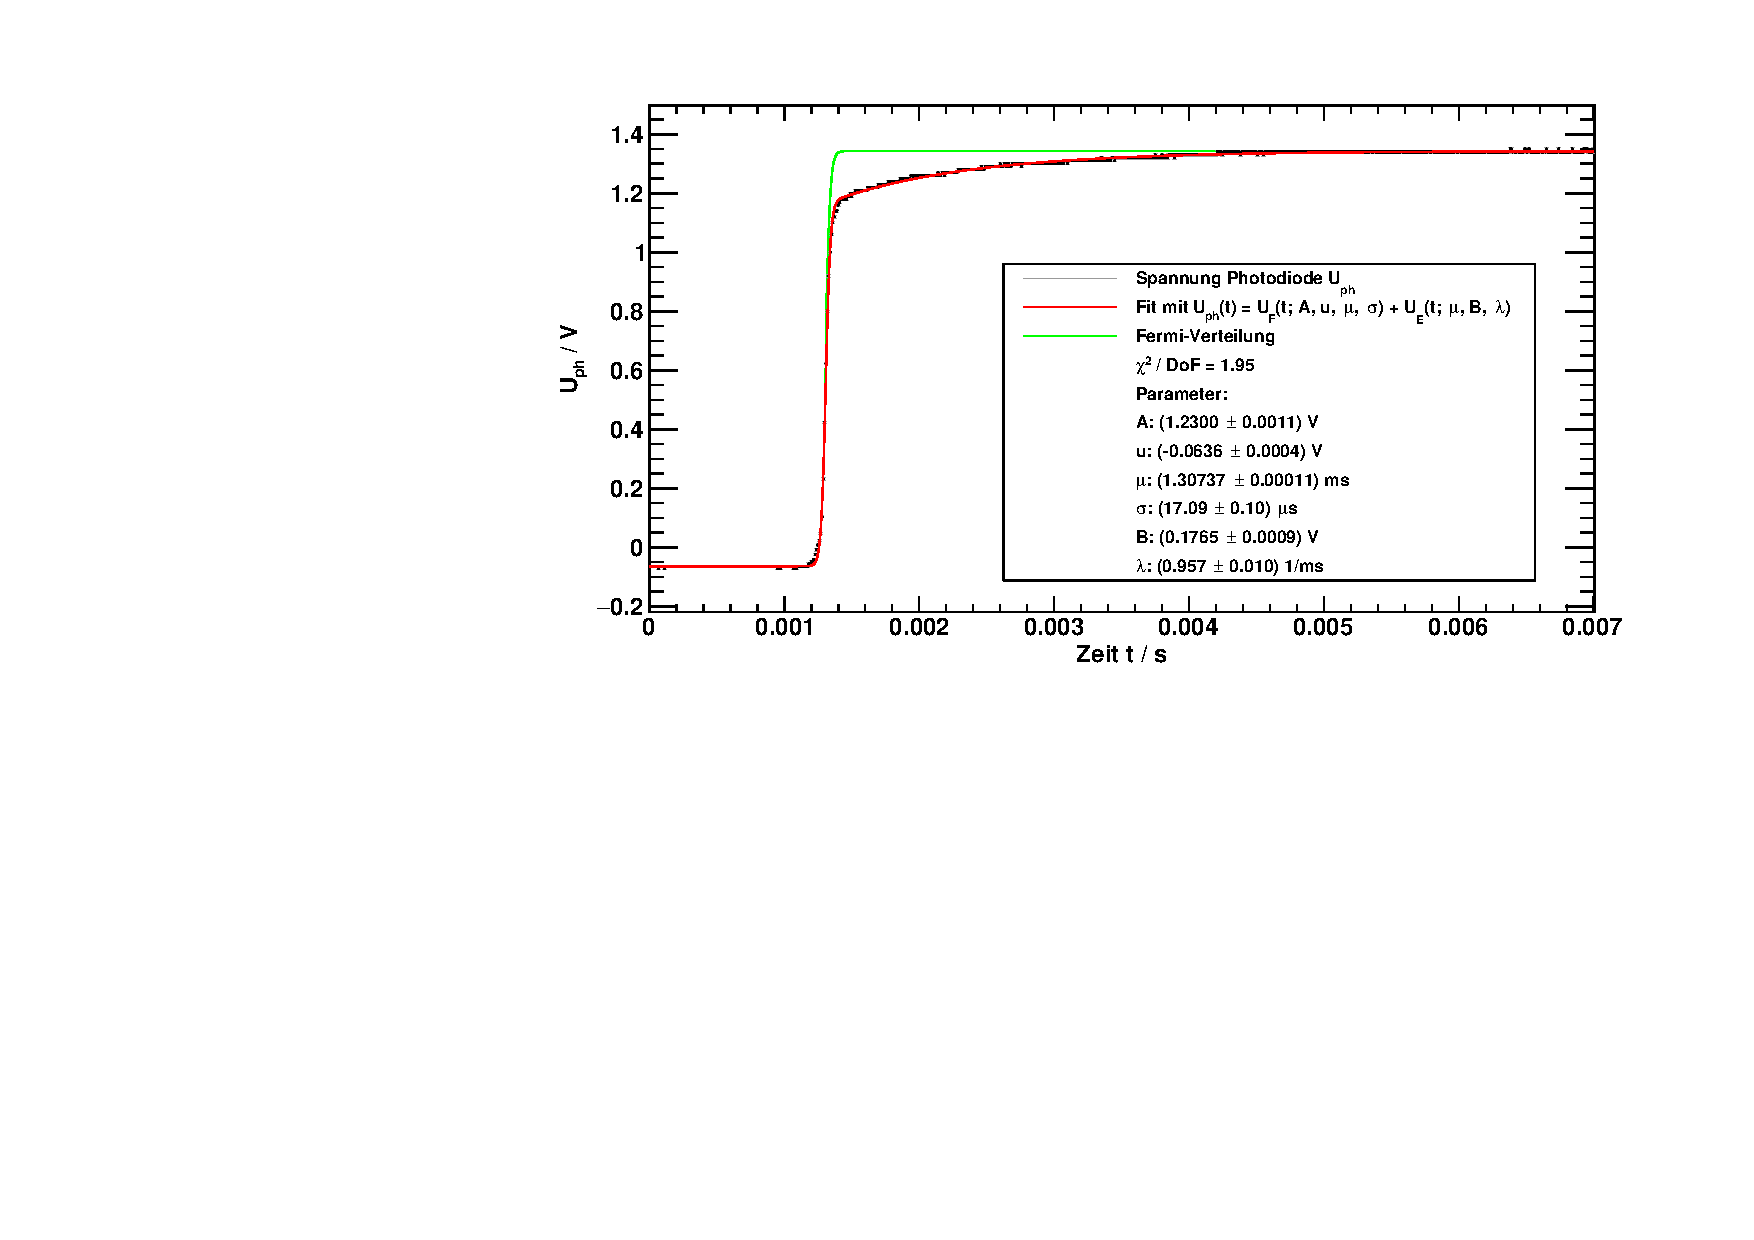
\includegraphics[width=\textwidth]{../img/part6/05.pdf}
        \caption{Transmission der Rubidiumzelle bei Einschalten des Laserlichts und Fit mit $U(t)$.
        Die Höhe der Delle $B$ am Anfang des Plateaus ist abhängig von der vorangehenden Dunkelzeit $t_\text{d}$
        und enthält die Information über das Ausmaß der Relaxation im Dunklen.}
        \label{img:fra:exampletrans}
    \end{center}
\end{figure}

Für die weitere Auswertung ist es notwendig, die Dunkelzeit $t_\text{d}$ zu bestimmen.
Die Methode dafür ist folgende:
Da die Chopperscheibe das Laserlicht mit einer Pulsweite von 50\% moduliert,
ist die Dunkelzeit genauso groß wie die Beleuchtungszeit.
Als Anfang der Beleuchtungszeit wird der gefittete Parameter $\mu$ verwendet.
Das Ende der Beleuchtungszeit $\mu'$ wird per Hand aus den Messdaten abgelesen
(es wird der Wert bei halber Transmission verwendet);
für den Fehler $s_{\mu'}$ auf die abgelesenen Werte wird
\begin{equation}
    s_{\mu'} = 0.01 \cdot \mu' + 0.1\,\text{ms}
\end{equation}
angenommen.
Es gilt dann für die Dunkelzeit
\begin{equation}
    t_\text{d}=\mu'-\mu \ \, .
\end{equation}

Eine Betrachtung der Fitergebnisse für die Verschmierung $\sigma$ der Fermi-Funktion
(\autoref{img:fra:sigmas}) zeigt,
warum es geeigneter ist, eine Fermi-Verteilung als Fitfunktion zu verwenden als ein
Rechtecksignal mit senkrechter Flanke:
Der nichtsenkrechte Anstieg des Rechtecksignals wird durch den Durchmesser des Laserstrahls verursacht, denn
der Strahl wird von der Chopperscheibe in einer kurzen Anstiegszeit geöffnet und nicht auf einmal.
Da die Anstiegszeit umgekehrt proportional zur Rotationsgeschwindigkeit der Scheibe und diese
wiederum umgekehrt proportional zur Dunkelzeit ist, erhält man einen linearen Zusammenhang
zwischen $\sigma$ und $t_\text{d}$.

Beim Experiment wurde versucht, die Anstiegszeit zu minimieren, indem der Chopper möglichst
nahe an die Laserdiode geschoben wurde, wo der Strahldurchmesser noch gering ist.

\begin{figure}[H]
    \begin{center}
        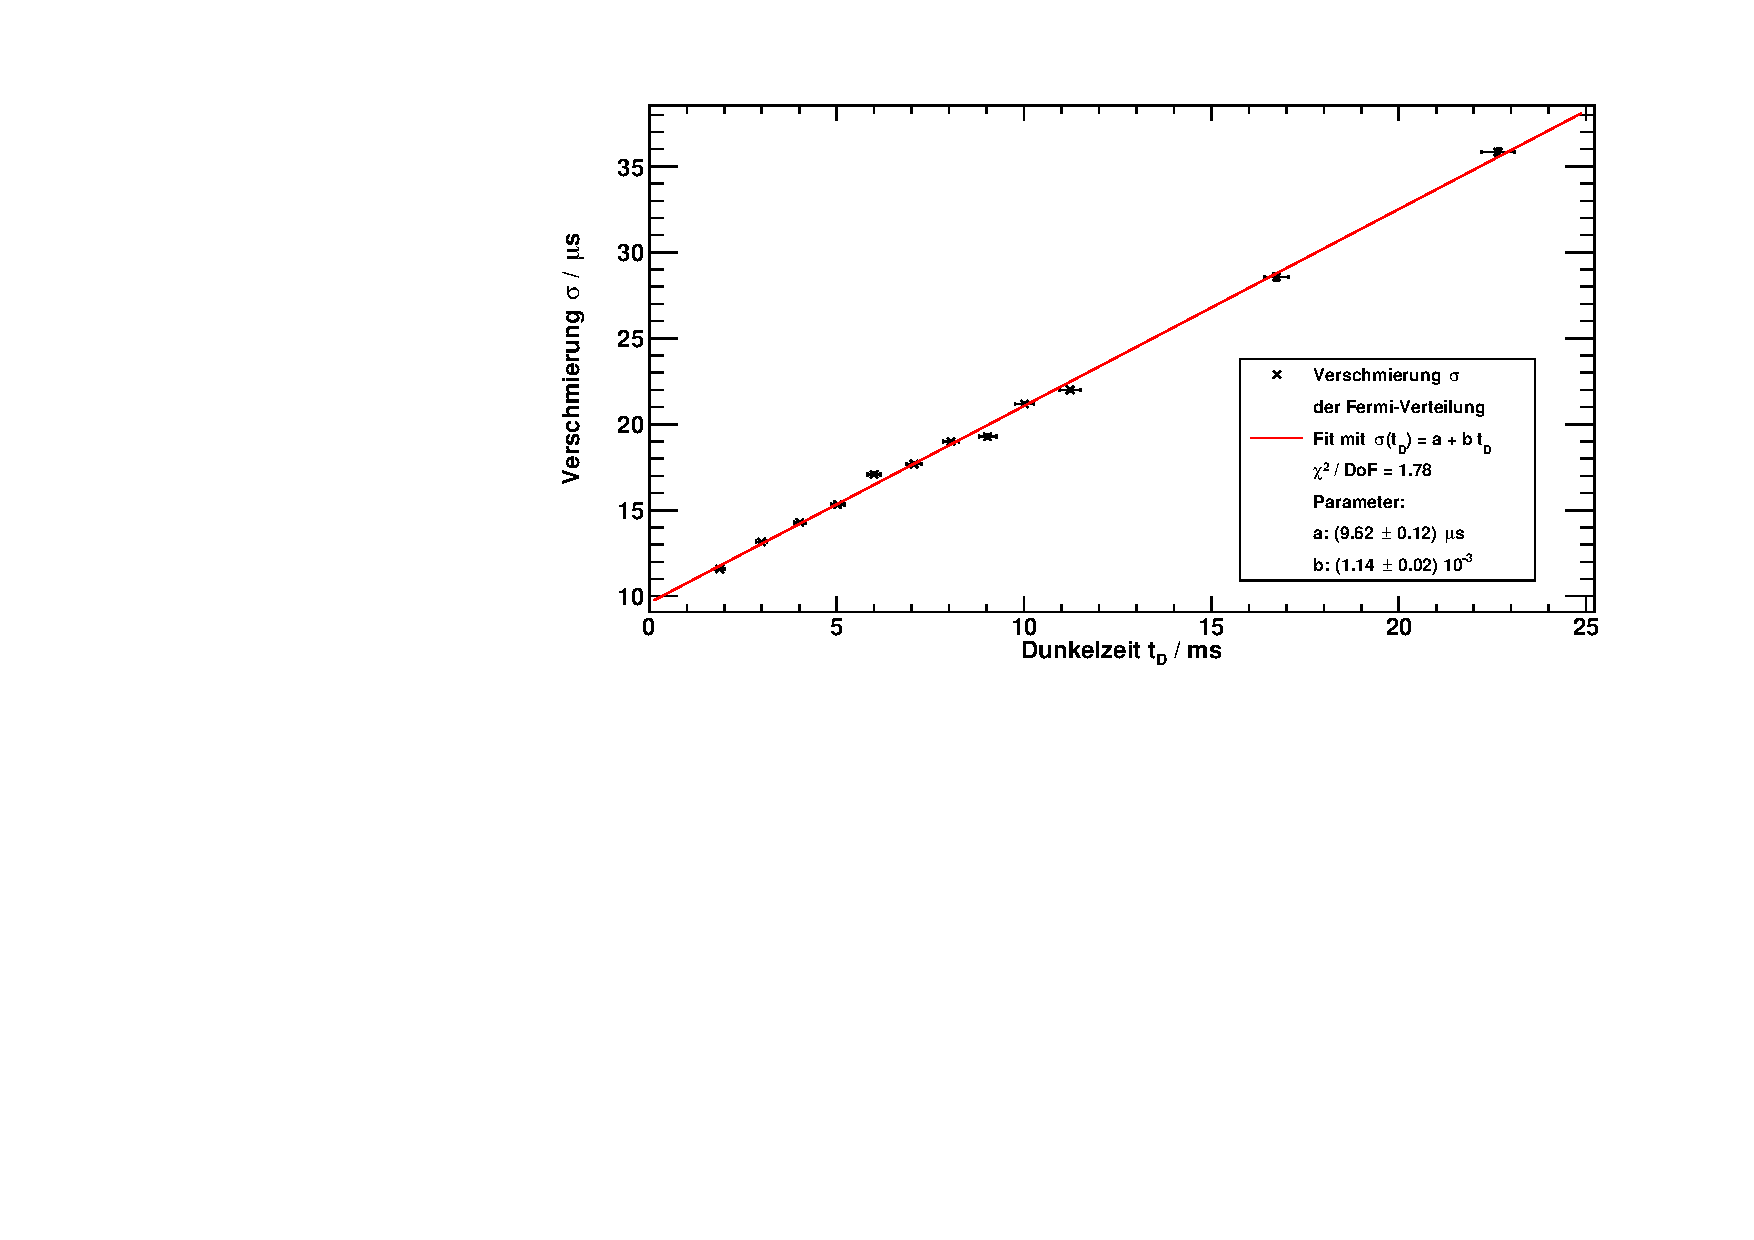
\includegraphics[width=\textwidth]{../img/part6/sigmaFit.pdf}
        \caption{Verschmierung $\sigma$ der gefitteten Fermi-Funktionen in Abhängigkeit der Dunkelzeit $t_\text{d}$.
        Ursache für den linearen Zusammenhang ist die kleinere Rotationsgeschwindigkeit des Choppers bei
        größeren Dunkelzeiten.}
        \label{img:fra:sigmas}
    \end{center}
\end{figure}

Der Wert für die Relaxationszeit $T_{\text{R}_\text{F}}$ kann aus den Fitdaten für den Parameter $B$ gewonnen werden.
Je größer die Dunkelzeit, desto länger kann das Ensemble relaxieren und $B$ ist dementsprechend größer.
Mit den Messungen bei unterschiedlichen Dunkelzeiten erhält
man daher Informationen über das Ausmaß der Relaxation zu
verschiedenen Zeitpunkten.
Die Relaxation folgt einem exponentiellen Gesetz; die Werte für $B$ werden daher mit
\begin{equation}
    B(t_\text{d})= a + b \cdot \left(1 - e^{-\frac{t_\text{d}}{T_{\text{R}_\text{F}}}}\right)
\end{equation}
gefittet.
\autoref{img:fra:Bs} zeigt diesen Fit. Der Parameter $a$ ist hier ein konstanter Offset,
$b$ beschreibt die Stärke der Relaxation bei großer Dunkelzeit und
$T_{\text{R}_\text{F}}$ die gesuchte Relaxationszeit nach Franzen.

\begin{figure}[H]
    \begin{center}
        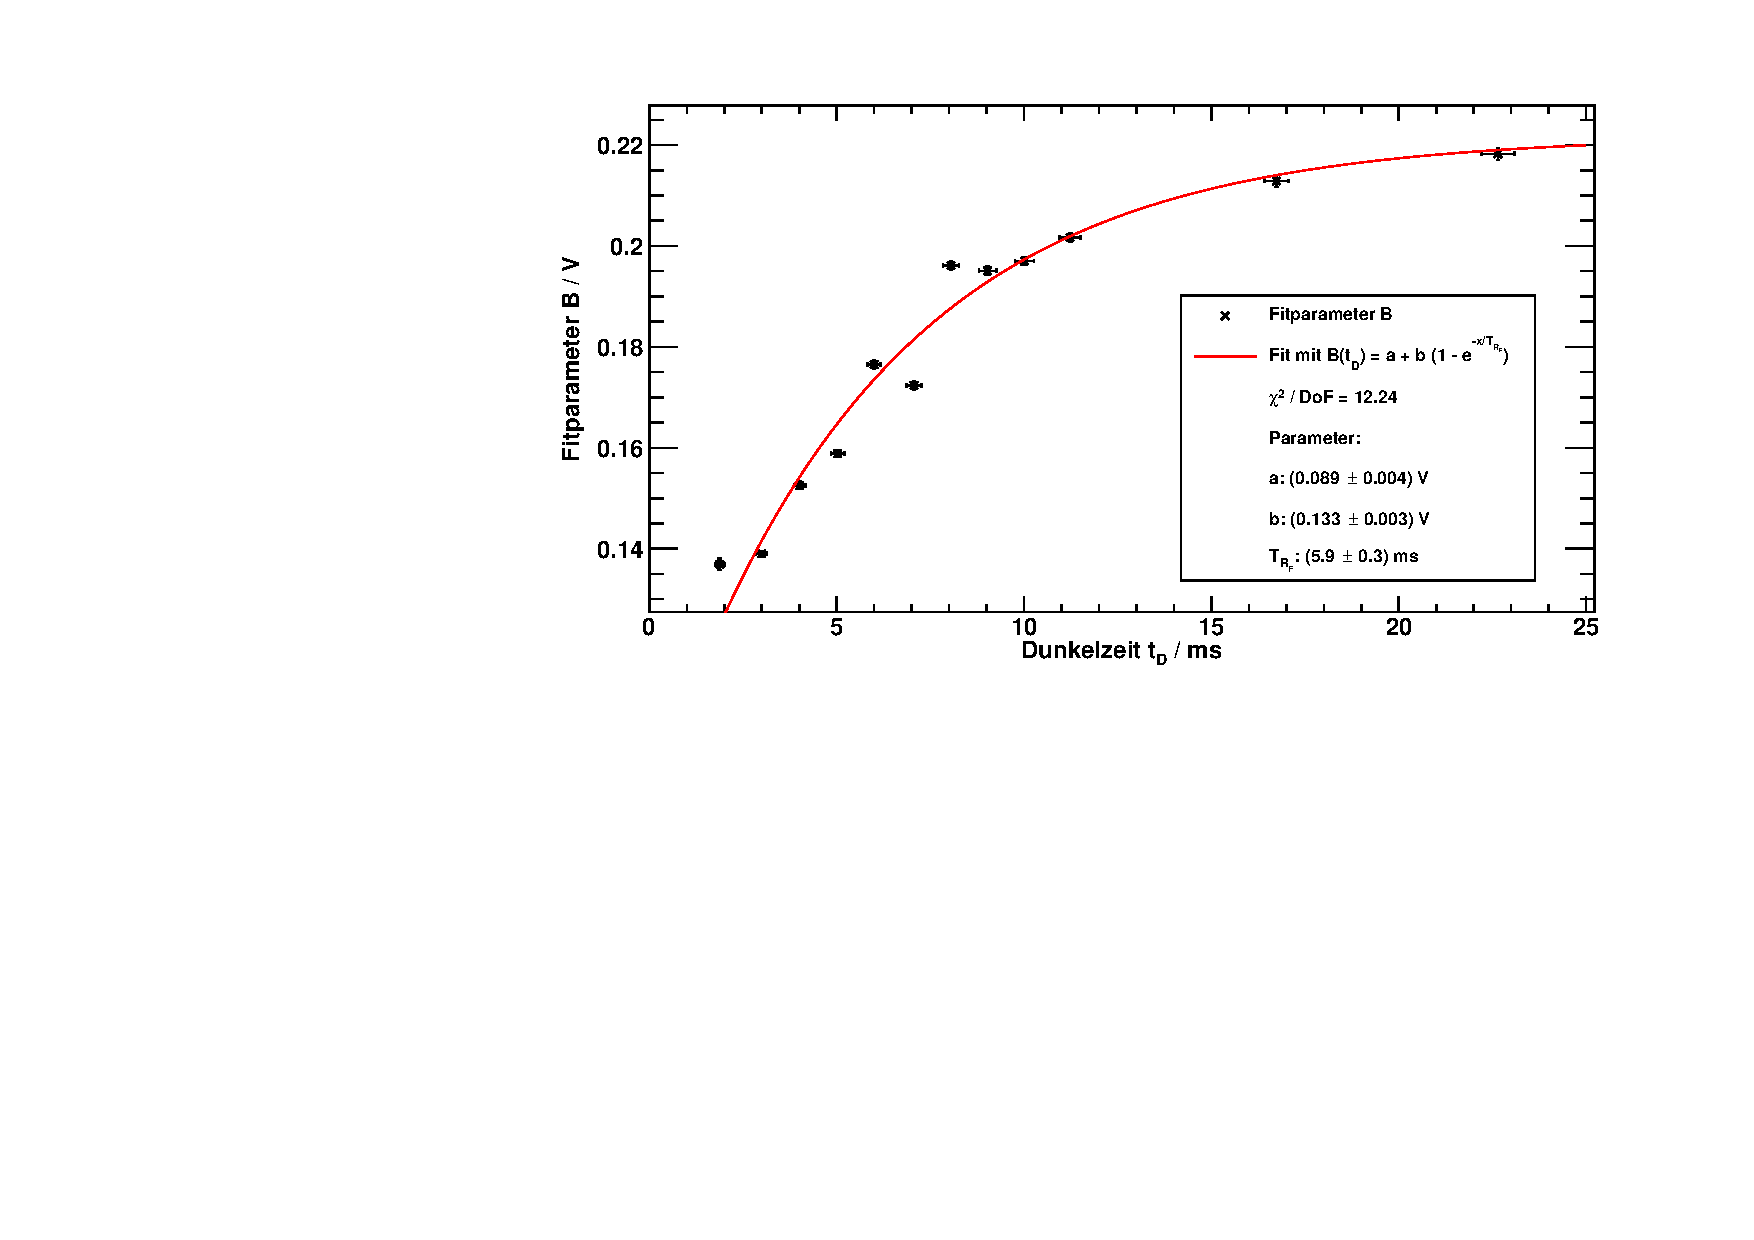
\includegraphics[width=\textwidth]{../img/part6/BFit.pdf}
        \caption{Abhängigkeit des Fitparameters $B$ aus \autoref{eq:fra:fitfunct} von der Dunkelzeit $t_\text{d}$ und Fit
        mit einer exponentiellem Gesetz zur Bestimmung der Relaxationszeit $T_{\text{R}_\text{F}}$.}
        \label{img:fra:Bs}
    \end{center}
\end{figure}

Der Fit liefert für die Relaxationszeit einen Wert von
\begin{equation}
    T_{\text{R}_\text{F}} = 5.9 \pm 0.3 \,\text{ms}  \ \, .
\end{equation}
Dieser Wert stimmt innerhalb von 2 Standardabweichungen mit dem theoretisch berechnetem Wert (\autoref{eq:tr:theo}) überein. 
Die Abweichung des experimentell bestimmen Wertes nach unten könnte durch die Spin-Spin-Relaxation erklärt werden, die vom theoretischen Modell 
nicht berücksichtigt wird.

\appendix
\section{Anhang}
\subsection{Messprotokoll}
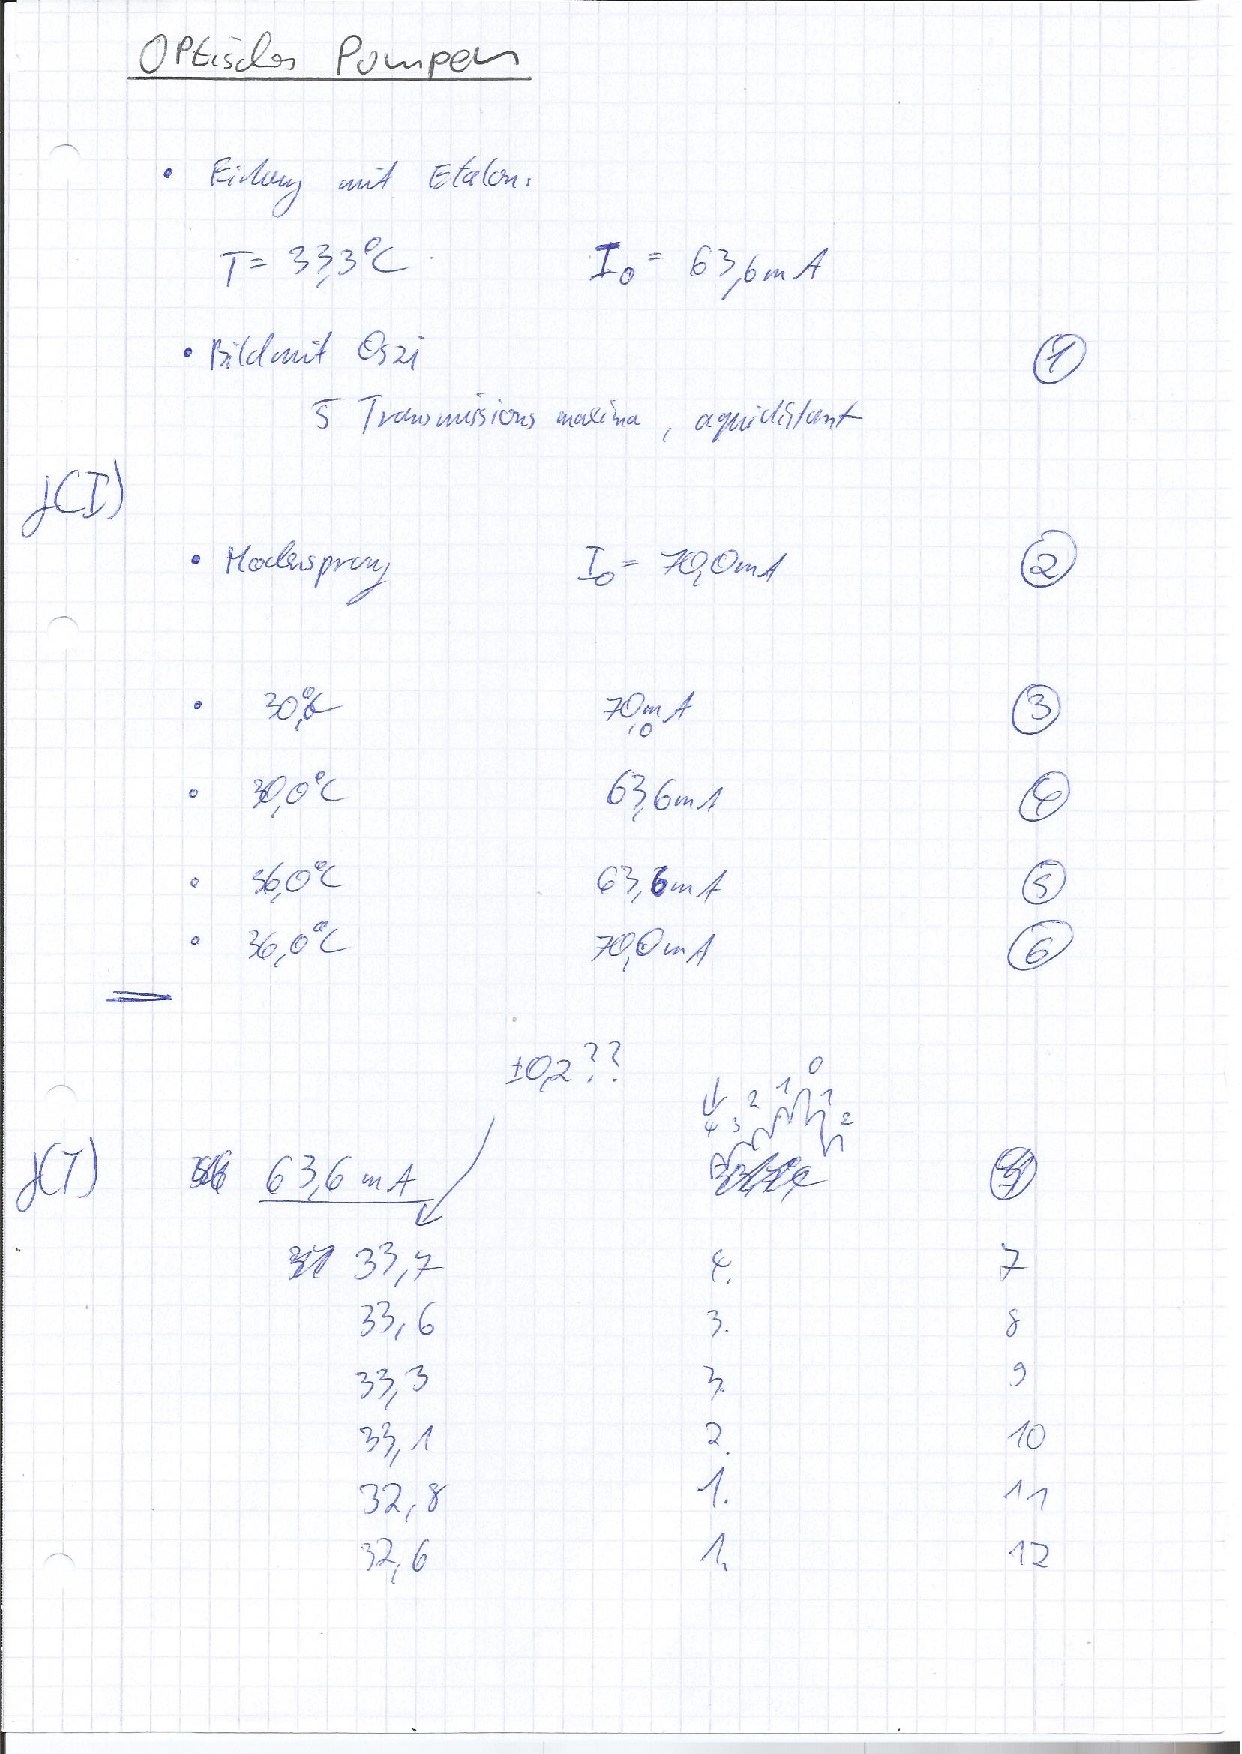
\includepdf[pages={-}]{../data/protokoll.pdf}


\end{document}